Στο κεφάλαιο αυτό παρουσιάζεται αναλυτικά η μελέτη της δυναμικής συμπεριφοράς ενός διακριτού συστήματος που αποτελεί παραλλαγή του γνωστού Λογιστικού Χάρτη. Για επιλεγμένες τιμές της παραμέτρου του μποροεί να παρουσιάσει χαοτική συμπεριφορά όπως και φαινόμενα που σχετίζονται με τη μη-γραμμική δυναμική. Για την μελέτη χρησιμοποιήθηκαν τα διαγράμματα διακλάδωσης, οι εκθέτες Lyapunov και οι απεικονίσεις της τιμής \(x_i\) σε συνάρτηση με  την τιμή \(x_{i+1}\).\\\\
%Στην ενότητα αυτή παρατίθεται η μελέτη ενός διακριτού συστήματος που αποτελεί παραλλαγή του γνωστού Λογιστικού Χάρτη. 
Ο Λογιστικός Χάρτης που αποτέλεσε τη βάση του προτεινόμενου σε αυτή την ενότητα, χάρτη, περιγράφεται από την παρακάτω εξίσωση:

\begin{equation}
	x_i=k*(1+x_{i-1})^2 *(2-x_{i-1})
	\label{f:x}
\end{equation}


Στην εξίσωση (\ref{f:x}) προστέθηκε ένας σταθερός όρος \emph{q}. Έτσι προέκυψε η προτεινόμενη παραλλαγή του Λογιστικού Χάρτη,

\begin{equation}
	x_i=k*(1+x_{i-1})^2 *(2-x_{i-1}) +q
	\label{f:x1}
\end{equation}
όπου \emph{k}, \emph{q} : παράμετροι.\\

Για την εύρεση της δυναμικής συμπεριφοράς του συστήματος εξετάστηκε μια περιοχή τιμών των συγκεκριμένων παραμέτρων, ώστε να επιτευχθεί ταυτόχρονη σύγκριση της περιοδικής και χαοτικής συμπεριφοράς του. Πιο συγκεκριμένα, στη μελέτη που πραγματοποιήθηκε η αρχική συνθήκη του $x_0 =0.1$ παρέμεινε  σταθερή, ενώ η τιμή της παραμέτρου \emph{q} μεταβαλλόταν στο διάστημα $[-0.1,-2.1]$. Στο διάστημα  $[-0.1,-0.9]$ και στο $[-1.2,-1.6]$ μεταβαλλόταν με βήμα $0.2$, ενώ στο $[-0.9,-1.2]$ και στο $[-1.6,-2.1]$ η παράμετρος  μεταβαλλόταν \emph{q} με βήμα $0.3$. Έτσι, για κάθε περίπτωση παράχθηκαν το διάγραμμα διακλάδωσης, το διάγραμμα των εκθετών Lyapunov και το διάγραμμα της τιμής \(x_i\) σε συνάρτηση με  την τιμή \(x_{i+1}\), τα οποία παρουσιάζονται και αναλύονται στη συνέχεια.\\


\section{Για q = -0.1 }

Στο Σχ. \ref{f:g1} παρατίθεται το διάγραμμα διακλάδωσης του συστήματος (\ref{f:x1}), ως προς την παράμετρο \emph{k}, για $q =- 0.1$. Για αυτές τις τιμές των παραμέτρων το σύστημα ξεκινάει από \emph{περίοδο - 1} για $k=0.3$, ενώ για  $k = 0.4$ εμφανίζει τον πρώτο διπλασιασμό της περιόδου. Τον δεύτερο διπλασιασμό τον εμφανίζει για $k=0.47$ (\emph{περίοδος - 4}), τον τρίτο για $k=0.476$  (\emph{περίοδος -   8}), ενώ ο τελευταίος διπλασιασμός εμφανίζεται λίγο πιο μετά τον τρίτο για k=0.478 (\emph{περίοδος - 16}). Στην συνέχεια για $k>0.479$ το σύστημα εισέρχεται στο χάος, μέχρι να εξέλθει για $k=0.51$ (\emph{περίοδος - 3}) και να ξανά εισέλθει στο χάος μετά από δύο διπλασιασμούς $k=0.52$ (\emph{περίοδος -   6}) και $k=0.522$ (\emph{περίοδος - 11}) για $k>0.524$. To φαινόμενο αυτό είναι γνωστό ως συνοριακή κρίση. Εξέρχεται για τελευταία φορά από το χάος για $k=0.555$ (\emph{περίοδος -   4}). Για $k=0.559$ εμφανίζεται ένας διπλασιασμός (\emph{περίοδος - 8}) ο οποίος καταστρέφεται για $k=0.568$, οπότε εδώ παρατηρούμε το φαινόμενο της αντιμονοτονικότητας δηλαδή έχουμε μία ανάστροφη ακολουθία διπλασιασμού της περιόδου για $k=0.568$. 

Λόγω αυτού του φαινομένου το οποίο συνεχίζει μέχρι το $q=-0.2$, μελετήθηκε περαιτέρω το σύστημα από $-0.1 < q < -0.2$. Τέλος για $k=0.5735$ έχουμε έναν τελευταίο διπλασιασμό (\emph{περίοδος - 6}) πριν ξανά εισέλθει το σύστημα για $k > 0.575$ στο χάος.
Στα Σχ. \ref{f:g211}, \ref{f:g2} παρατίθενται 4 διαγράμματα διακλάδωσης 
(\ref{f:g3}, \ref{f:g4}, \ref{f:g5}, \ref{f:g6})
για $0.54<k<0.6$. Ουσιαστικά εστιάστηκε το διάγραμμα στην αντιμονοτονικότητα που εμφανίζεται για τις συγκεκριμένες τιμές του \emph{q}. Επίσης παρατηρούμε στα διαγράμματα \ref{f:g4}, \ref{f:g5}, \ref{f:g6} τη δημιουργία χαοτικών φυσαλίδων. Δηλαδή, το σύστημα εισέρχεται στο χάος με διπλασιασμό της περιόδου και στην συνέχεια εξέρχεται από αυτό με αντίστροφο διπλασιασμό της περιόδου. Επιπλέον στο διάγραμμα \ref{f:g6} το φαινόμενο εμφανίζεται δυο φορές  για $0.560<k<0.568$ και $0.571<k<0.573$. 

Επιπλέον, στο Σχ. \ref{f:g7} παρατίθεται το διάγραμμα των εκθετών Lyapunov για τιμές του \emph{k} στο ίδιο διάστημα τιμών $[0.3, 0.6]$. Στο διάστημα τιμών   $k=0.522$, στο $0.51<k<0.522$, και στο $0.554<k<0.574$ παρατηρούμε ότι το διάγραμμα των εκθετών Lyapunov είναι συνεχώς αρνητικός, γεγονός που επιβεβαιώνει την περιοδική συμπεριφορά του συστήματος. Ενώ στα υπόλοιπα διαστήματα ο θετικός εκθέτης Lyapunov υποστηρίζει την χαοτική του συμπεριφορά, όπως έγινε φανερό και από το διάγραμμα διακλάδωσης.

Τέλος, στον πίνακα \ref{tab:abc} παρατίθενται ενδεικτικές τιμές της παραμέτρου \emph{k} και η συμπεριφορά που παρουσιάζει το σύστημα για αυτές, σύμφωνα με το διάγραμμα διακλάδωσης, καθώς και τα αντίστοιχα σχήματα των διαγραμμάτων της τιμής \(x_i\) σε συνάρτηση με την τιμή \(x_{i+1}\). Από τα παραγόμενα σχήματα προκύπτει αριθμός σημείων αντίστοιχος με την περίοδο του συστήματος.\\\\


\begin{table}[ht]
	\centering
	\caption{Συμπεριφορά του υπό μελέτη συστήματος για διάφορες τιμές του \emph{k}, για $q=-0.1$.}
	\begin{tabular}{l | l | l}
		Παράμετρος k & Συμπεριφορά & Σχήμα\\
		\hline
		0.3 &  Περίοδος - 1 & \ref{f:k1}\\
		0.41 & Περίοδος - 2 & \ref{f:k2}\\
		0.476 &  Περίοδος - 8 & \ref{f:k3}\\
		0.4778 & Περίοδος - 16 & \ref{f:k4}\\
		0.479 & Χάος & \ref{f:k5}\\
		0.517 & Περίοδος - 3 & \ref{f:k6}\\
		0.521 & Περίοδος - 6 & \ref{f:k7}\\
		0.522 & Περίοδος - 11 & \ref{f:k8}\\
		0.524 & Χάος & \ref{f:k9}\\
		0.555 & Περίοδος - 4 & \ref{f:k10}\\
		0.559 & Περίοδος - 8 & \ref{f:k11}\\
		0.568 & Περίοδος - 4 & \ref{f:k12}\\
		0.5735 & Περίοδος - 6 & \ref{f:k13}\\
		0.575 & Χάος & \ref{f:k14}\\
	\end{tabular}
	
	\label{tab:abc}
\end{table}


\begin{figure}[ht]
	\centering
	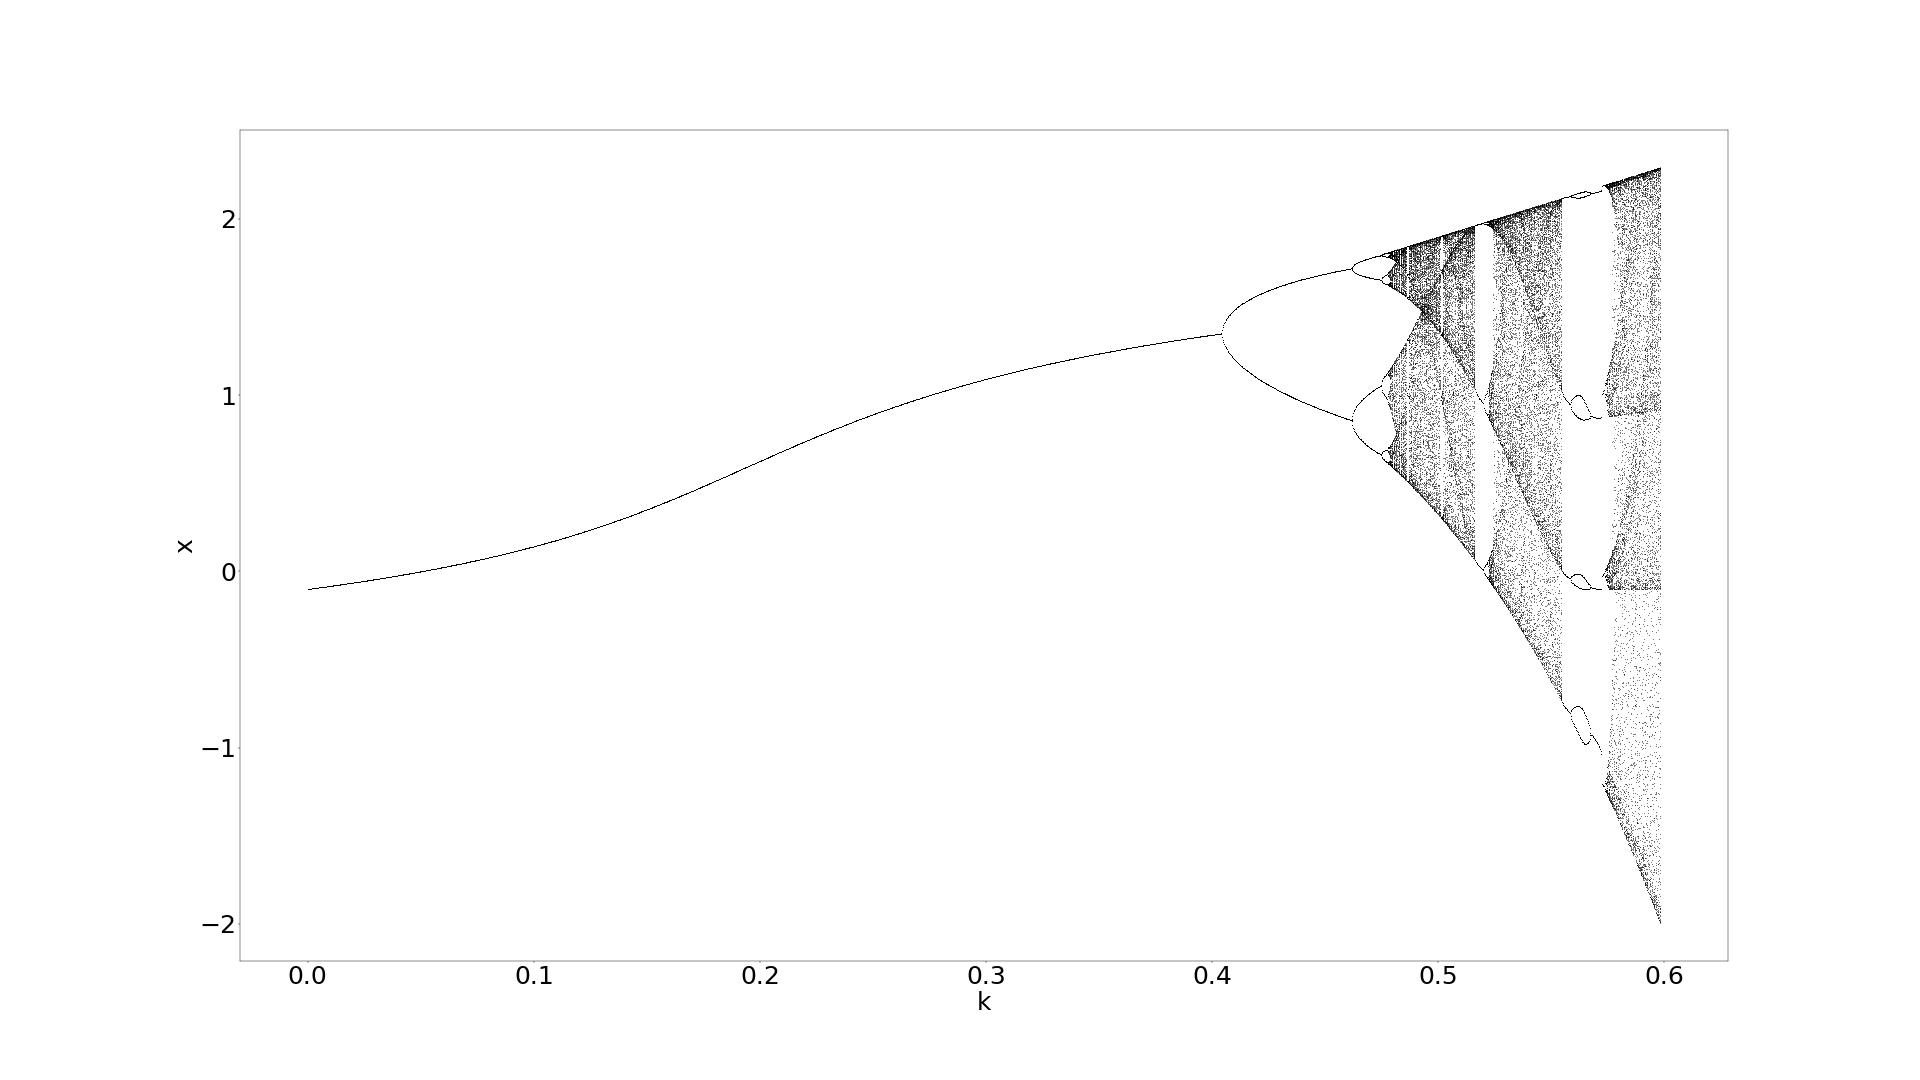
\includegraphics[width=1\linewidth]{LateX images/graphs/g1}
	\caption{ Διάγραμμα διακλάδωσης, για $q=-0.1$.}
	\label{f:g1}	
\end{figure}

\begin{figure}[ht]
	\centering
	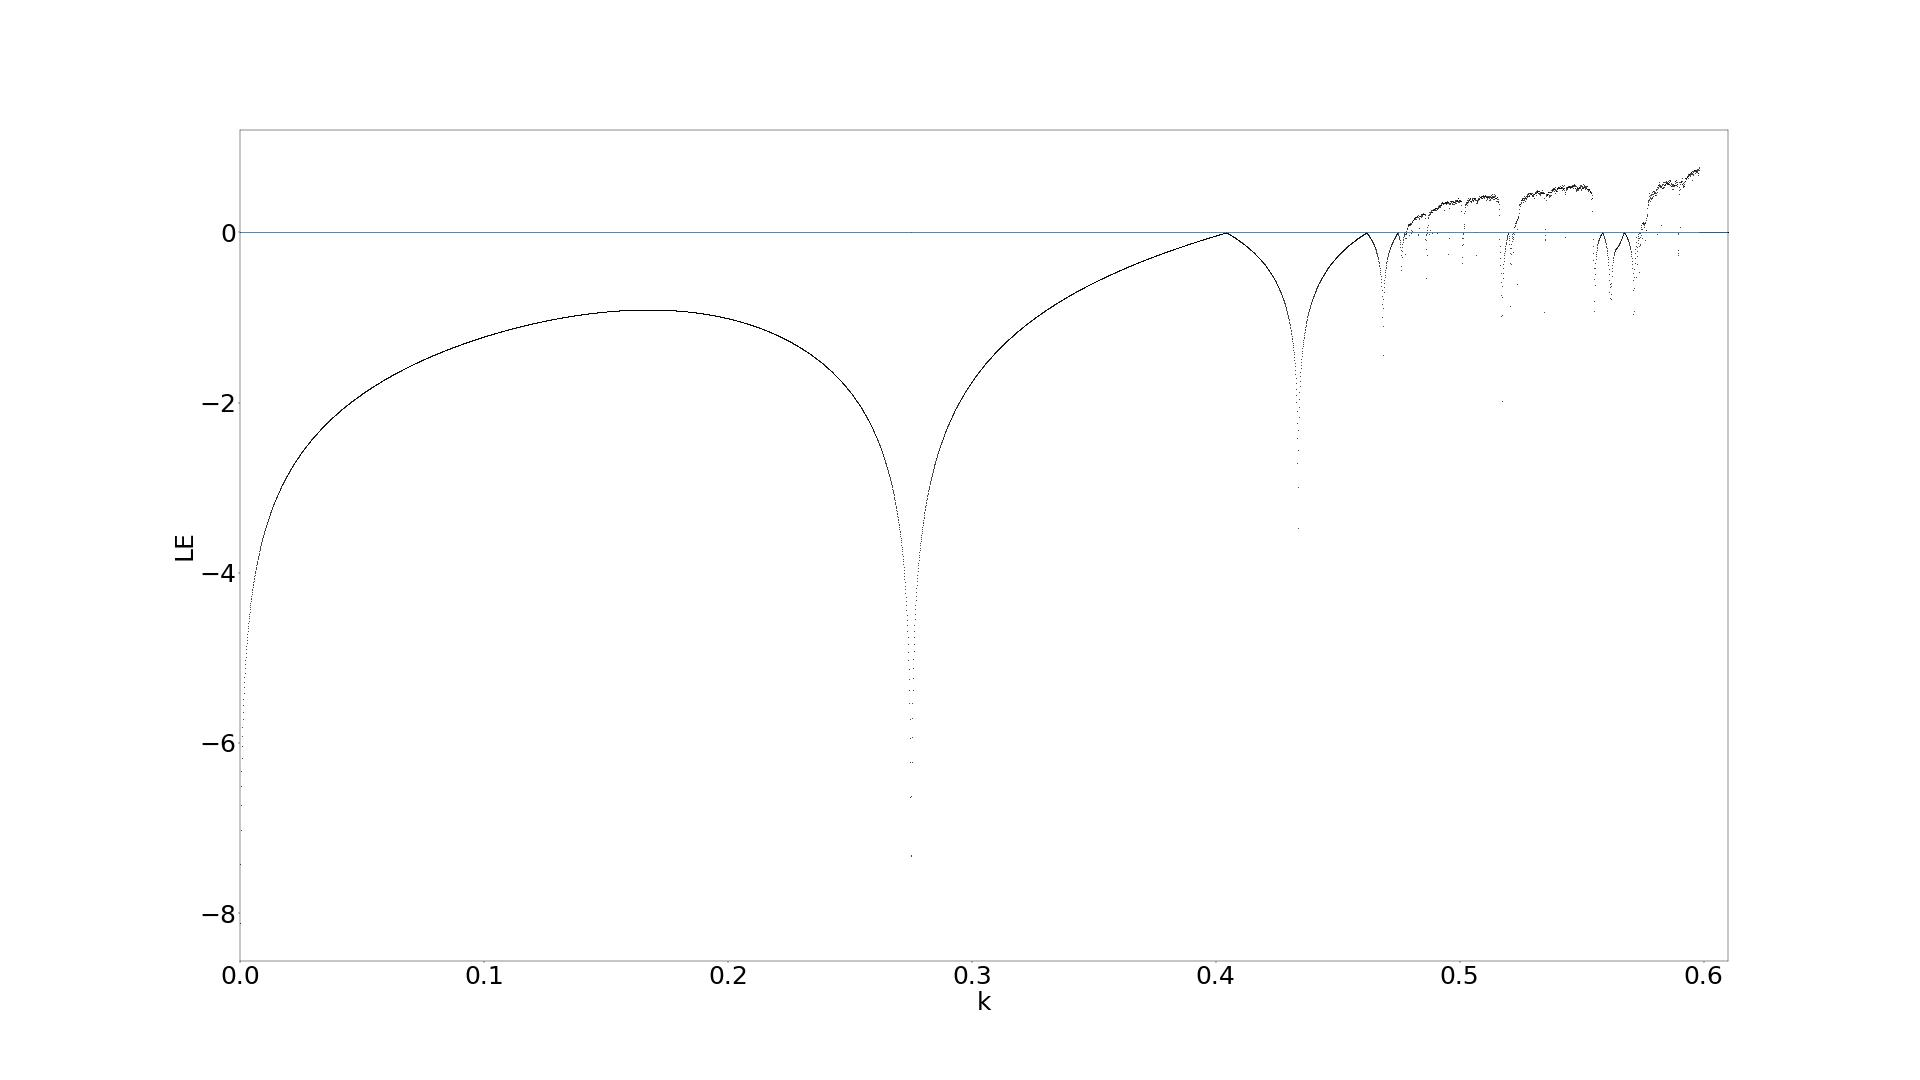
\includegraphics[width=1\linewidth]{LateX images/graphs/g2}
	\caption{Διάγραμμα των εκθετών Lyapunov σε συνάρτηση με την παράμετρο \emph{k}, για $q=-0.1$.}
	\label{f:g7}
\end{figure}


\begin{figure}[ht]
	\centering
	
	\begin{subfigure}[b]{1\textwidth}
		\centering
		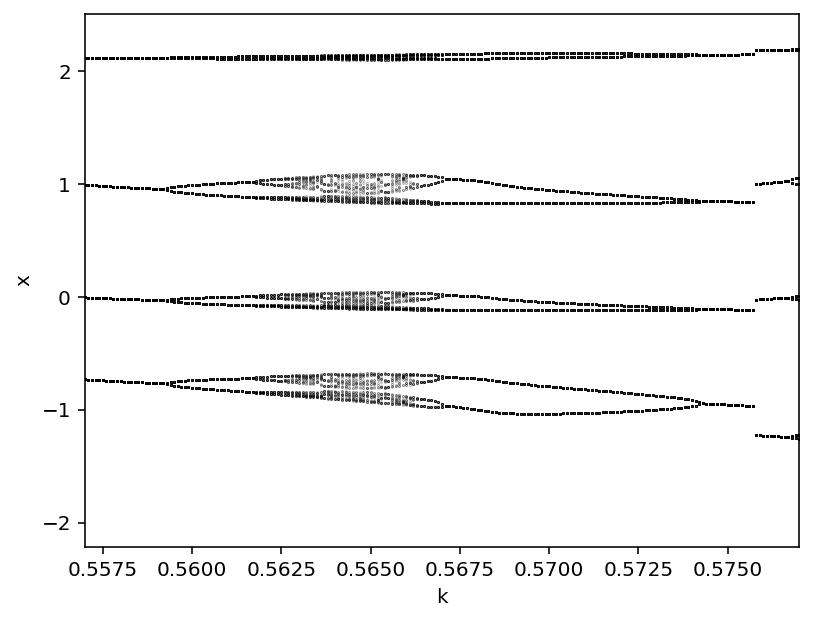
\includegraphics[width=\textwidth]{LateX images/graphs/g3}
		\caption{Για $q=-0.112$}
		\label{f:g3}
	\end{subfigure}
	\hfill
	\begin{subfigure}[b]{1\textwidth}
		\centering
		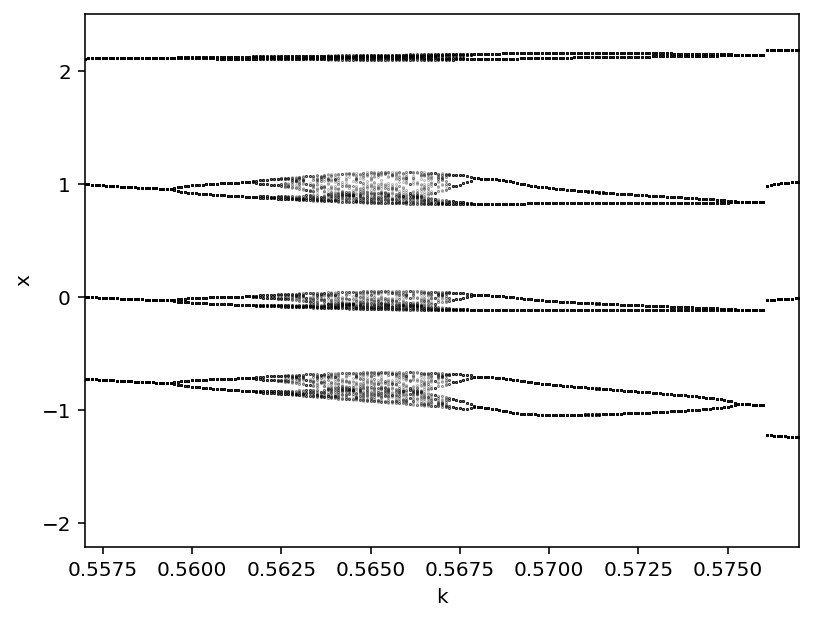
\includegraphics[width=\textwidth]{LateX images/graphs/g4}
		\caption{Για $q=-0.114$}
		\label{f:g4}
	\end{subfigure}
	\hfill
	\caption{Διαγράμματα διακλάδωσης για διάφορες τιμές του $q$ (α' μέρος). }
\label{f:g211}
\end{figure}
	
\begin{figure}[ht]
	\centering
	\begin{subfigure}[b]{1\textwidth}
		\centering
		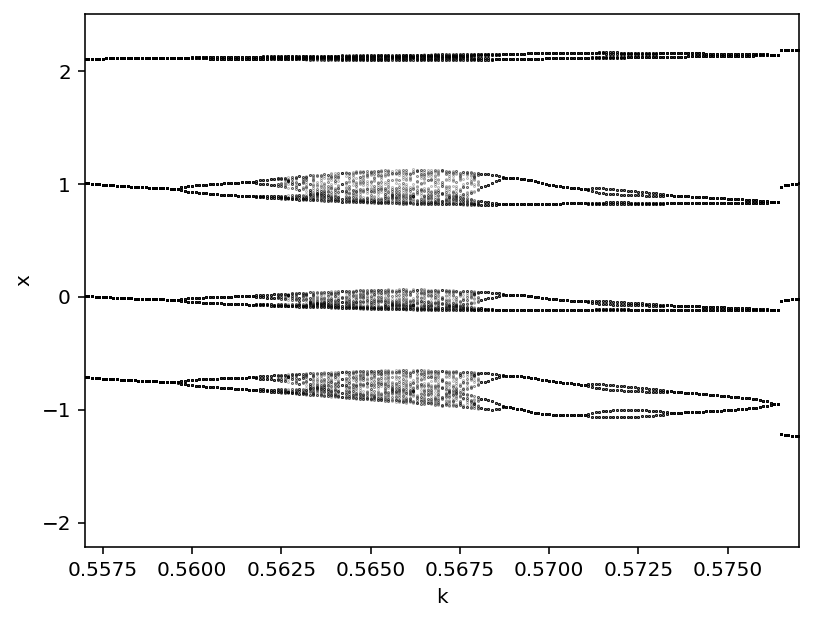
\includegraphics[width=\textwidth]{LateX images/graphs/g5}
		\caption{Για $q=-0.116$}
		\label{f:g5}
	\end{subfigure}
	\hfill
	\begin{subfigure}[b]{1\textwidth}
		\centering
		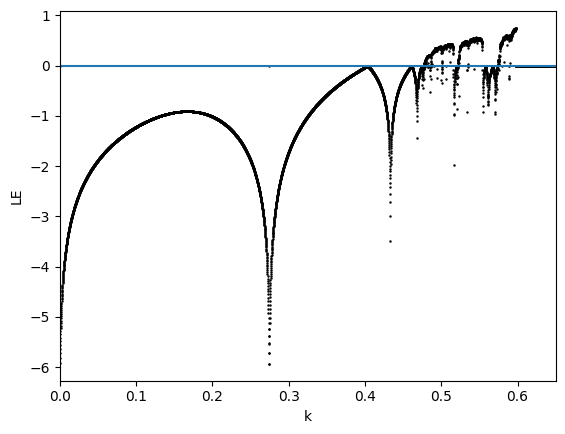
\includegraphics[width=\textwidth]{LateX images/graphs/g6}
		\caption{Για $q=-0.118$}
		\label{f:g6}
	\end{subfigure}
	
\caption{Διαγράμματα διακλάδωσης για διάφορες τιμές του $q$ (β' μέρος). }
\label{f:g2}
\end{figure}



\begin{figure}[ht]
	\centering	
	\begin{subfigure}[b]{0.4\linewidth}
		\centering
		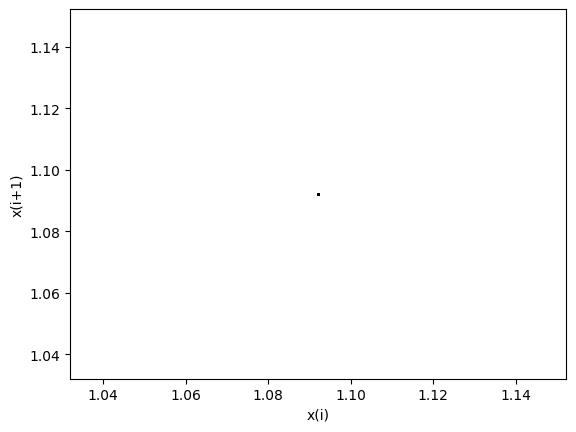
\includegraphics[width=\linewidth]{LateX images/graphs/k03}
		\caption{Για $k=0.3$}
		\label{f:k1}
	\end{subfigure}
	\hfill
	\begin{subfigure}[b]{0.4\textwidth}
		\centering
		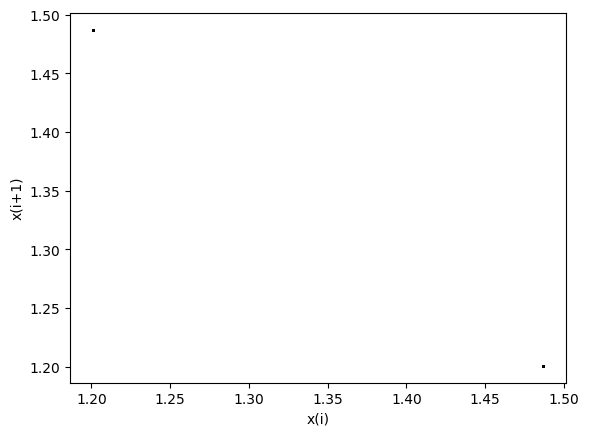
\includegraphics[width=\textwidth]{LateX images/graphs/k041}
		\caption{Για $k=0.41$}
		\label{f:k2}
	\end{subfigure}
	\hfill
	\begin{subfigure}[b]{0.4\textwidth}
		\centering
		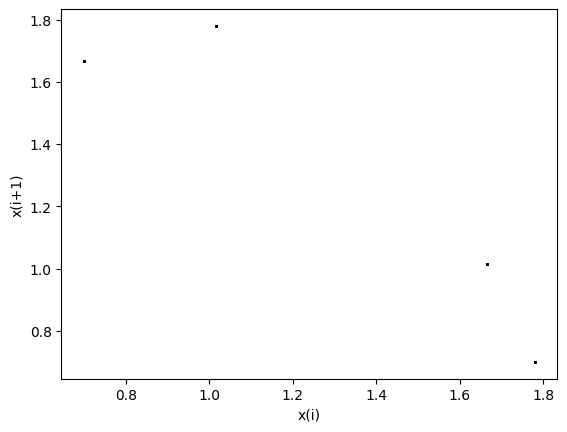
\includegraphics[width=\textwidth]{LateX images/graphs/k047}
		\caption{Για $k=0.047$}
		\label{f:k3}
	\end{subfigure}
	\hfill
	\begin{subfigure}[b]{0.4\textwidth}
		\centering
		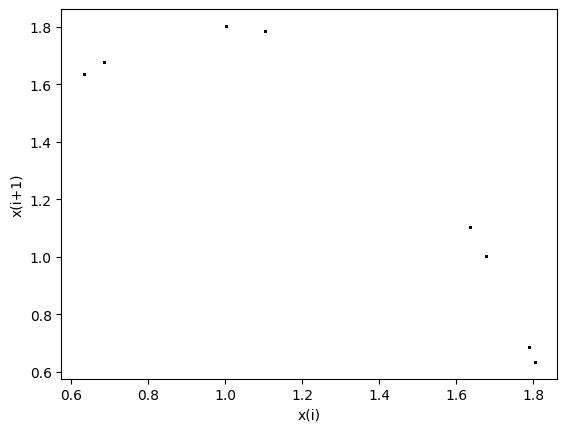
\includegraphics[width=\textwidth]{LateX images/graphs/k0476}
		\caption{Για $k=0.476$}
		\label{f:k4}
	\end{subfigure}
	\hfill
	\begin{subfigure}[b]{0.4\textwidth}
		\centering
		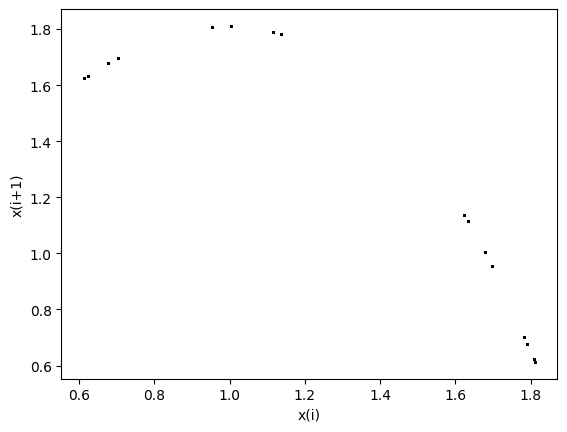
\includegraphics[width=\textwidth]{LateX images/graphs/k04778}
		\caption{Για $k=0.4778$}
		\label{f:k5}
	\end{subfigure}
	\hfill
	\begin{subfigure}[b]{0.4\textwidth}
		\centering
		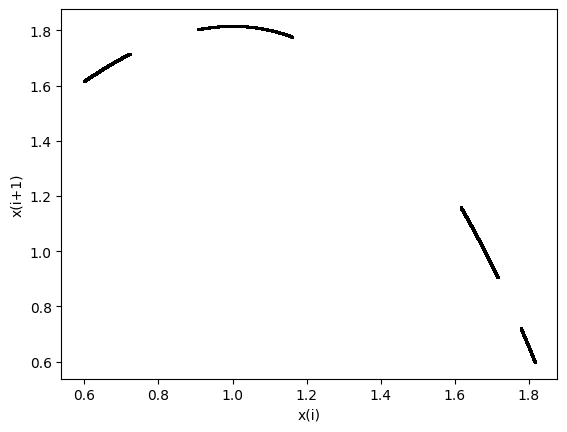
\includegraphics[width=\textwidth]{LateX images/graphs/k0479}
		\caption{Για $k=0.479$}
		\label{f:k6}
	\end{subfigure}
	\hfill	
	\begin{subfigure}[b]{0.4\textwidth}
		\centering
		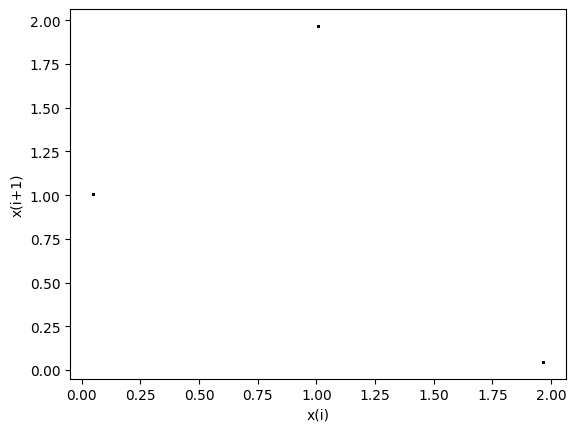
\includegraphics[width=\textwidth]{LateX images/graphs/k0517}
		\caption{Για $k=0.517$}
	\end{subfigure}
	\hfill
	\begin{subfigure}[b]{0.4\textwidth}
		\centering
		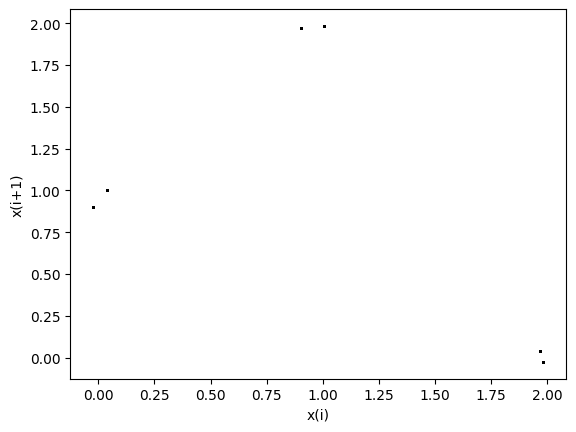
\includegraphics[width=\textwidth]{LateX images/graphs/0.521}
		\caption{Για $k=0.521$}
		\label{f:k7}
	\end{subfigure}
	\hfill
	\caption{Διαγράμματα της τιμής \(x_i\) με την τιμή \(x_{i+1}\) (α' μέρος).}
\end{figure}

\begin{figure}[ht]
	\centering
	\begin{subfigure}[c]{0.4\textwidth}
		\centering
		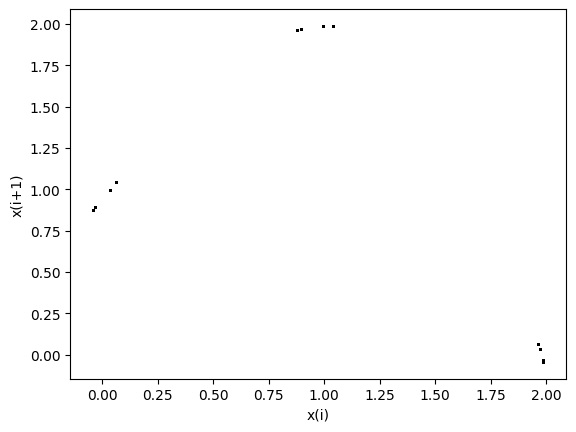
\includegraphics[width=\textwidth]{LateX images/graphs/k0522}
		\caption{Για $k=0.522$}
		\label{f:k8}
	\end{subfigure}
	\hfill
	\begin{subfigure}[c]{0.4\textwidth}
		\centering
		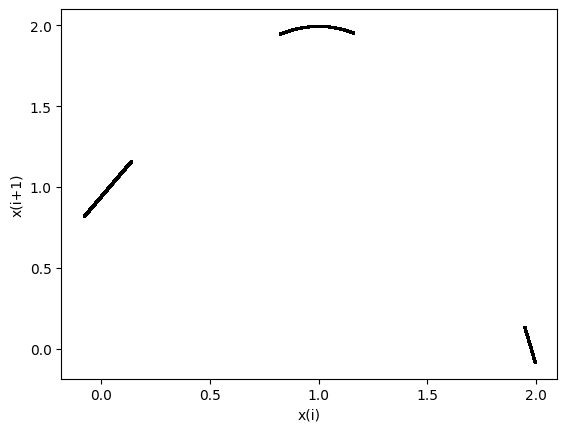
\includegraphics[width=\textwidth]{LateX images/graphs/k0524}
		\caption{Για $k=0.524$}
		\label{f:k9}
	\end{subfigure}
	\hfill
	\begin{subfigure}[c]{0.4\textwidth}
		\centering
		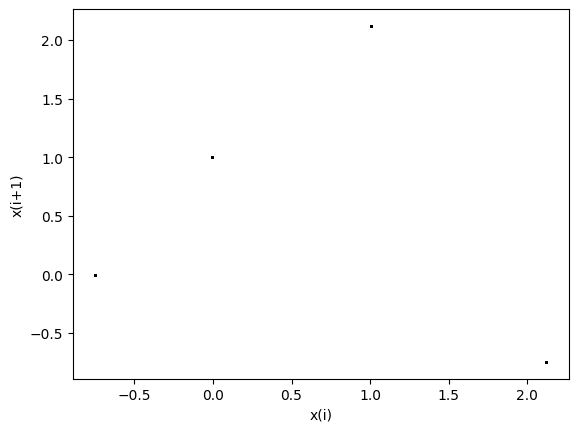
\includegraphics[width=\textwidth]{LateX images/graphs/k0555}
		\caption{Για $k=0.555$}
		\label{f:k10}
	\end{subfigure}
	\hfill
	\begin{subfigure}[c]{0.4\textwidth}
		\centering
		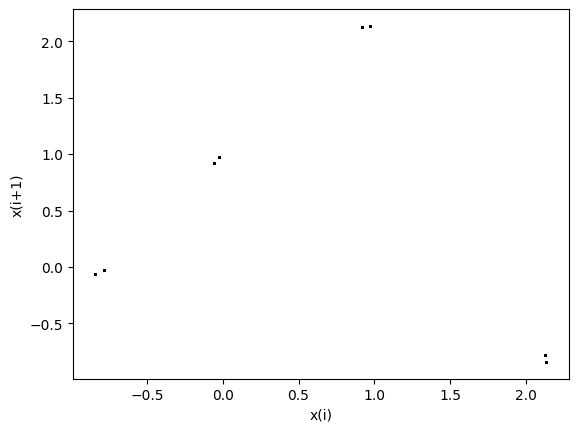
\includegraphics[width=\textwidth]{LateX images/graphs/k0559}
		\caption{Για $k=0.559$}
		\label{f:k11}
	\end{subfigure}
	\hfill
	\begin{subfigure}[c]{0.4\textwidth}
		\centering
		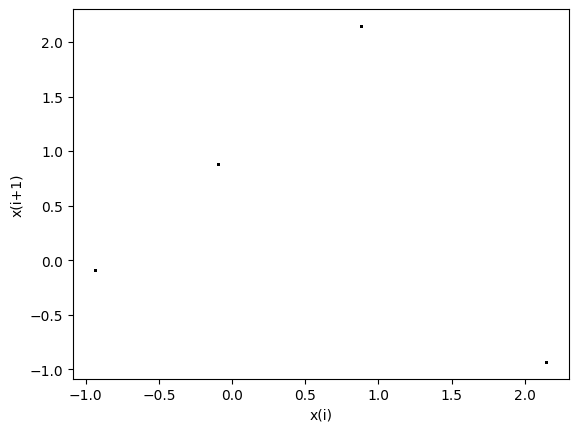
\includegraphics[width=\textwidth]{LateX images/graphs/k0568}
		\caption{Για $k=0.568$}
		\label{f:k12}
	\end{subfigure}
	\hfill
	\begin{subfigure}[c]{0.4\textwidth}
		\centering
		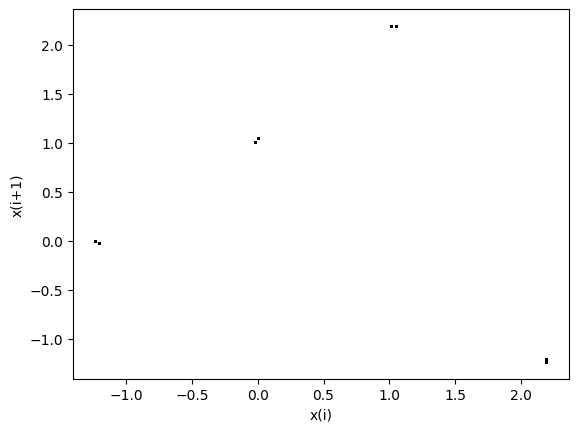
\includegraphics[width=\textwidth]{LateX images/graphs/k05735}
		\caption{Για $k=0.5735$}
		\label{f:k13}
	\end{subfigure}
	\hfill
	\begin{subfigure}[c]{0.4\textwidth}
		\centering
		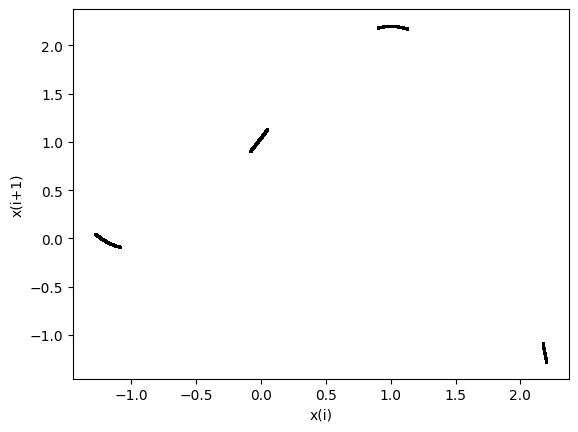
\includegraphics[width=\textwidth]{LateX images/graphs/k0575}
		\caption{Για $k=0.575$}
		\label{f:k14}
	\end{subfigure}
	\caption{Διαγράμματα της τιμής \(x_i\) σε συνάρτηση με την τιμή \(x_{i+1}\) (β' μέρος).}
\end{figure}
\vfill
\clearpage
\newpage
\section{Για q = -0.3}

Στο Σχ. \ref{f:g8} παρατίθεται το διάγραμμα διακλάδωσης του συστήματος (\ref{f:x1}), ως προς την παράμετρο \emph{k}, για $q =-0.3$. Για αυτές τις τιμές των παραμέτρων το σύστημα ξεκινάει από \emph{περίοδο - 1} για $k=0.3$, ενώ για  $k = 0.44$ εμφανίζει τον πρώτο διπλασιασμό της περιόδου. Τον δεύτερο διπλασιασμό τον εμφανίζει για $k=0.5$ (\emph{περίοδος -   4}), τον τρίτο για $k=0.511$ (\emph{περίοδος -   8}). Στην συνέχεια για $k>0.5165$ το σύστημα εισέρχεται στο χάος, μέχρι να εξέλθει  για $k=0.551$ (\emph{περίοδος -   3}) και να ξανά εισέλθει σε χάος μετά από δύο διπλασιασμούς $k=0.555$ (\emph{περίοδος - 6}) και $k=0.556$ (\emph{περίοδος - 12}) για $k>0.5573$. Επομένως, εμφανίζει πάλι τη συνοριακή κρίση. Εξέρχεται για τελευταία φορά από το χάος για $k=0.583$ (\emph{περίοδος - 4}) και μετά απο ένα διπλασιασμό  για $k=0.5846$ (\emph{περίοδος - 7}) εισέρχεται για τελευταία φορά στο χάος για $k=0.5851$.
Επομένως και σε αυτή την περίπτωση το σύστημα εισέρχεται στο χάος με διπλασιασμό της περιόδου. 

Επιπλέον, στο Σχ. \ref{f:g9} παρατίθεται το διάγραμμα των εκθετών Lyapunov για τιμές του \emph{k} στο ίδιο διάστημα τιμών $[0, 0.636]$. Στο διάστημα τιμών   $0<k<0.511$ , στο $0.551<k<0.556$, και στο $0.583<k<0.5846$ παρατηρούμε ότι το διάγραμμα των εκθετών Lyapunov είναι συνεχώς αρνητικός, γεγονός που επιβεβαιώνει την περιοδική συμπεριφορά του συστήματος. Ενώ στα υπόλοιπα διαστήματα ο θετικός εκθέτης Lyapunov υποστηρίζει την χαοτική του συμπεριφορά, όπως έγινε φανερό και από το διάγραμμα διακλάδωσης.

Τέλος, στον πίνακα \ref{tab:abc1} παρατίθενται ενδεικτικές τιμές της παραμέτρου \emph{k} και η συμπεριφορά που παρουσιάζει το σύστημα για αυτές, σύμφωνα με το διάγραμμα διακλάδωσης, καθώς και τα αντίστοιχα σχήματα των διαγραμμάτων της τιμής \(x_i\) σε συνάρτηση με την τιμή \(x_{i+1}\). Από τα παραγόμενα σχήματα προκύπτει αριθμός σημείων αντίστοιχος με την περίοδο του συστήματος.\\\\

\begin{table}[ht]
	\centering
	\caption{ Συμπεριφορά του υπό μελέτη συστήματος για διάφορες τιμές του \emph{k}, για $q=-0.3$.}
	\label{tab:abc1}
	\begin{tabular}{l | l | l}
		Παράμετρος k & Συμπεριφορά & Σχήμα\\
		\hline
		0.3 &  Περίοδος - 1 & \ref{f:k1}\\
		0.44& Περίοδος - 2 & \ref{f:k2}\\
		0.5& Περίοδος - 4 & \ref{f:k2}\\
		0.511 &  Περίοδος - 8 & \ref{f:k3}\\
		0.5165 & Χάος & \ref{f:k5}\\
		0.551 & Περίοδος - 3 & \ref{f:k6}\\
		0.555 & Περίοδος - 6 & \ref{f:k7}\\
		0.556 & Περίοδος - 12 & \ref{f:k8}\\
		0.5573 & Χάος & \ref{f:k9}\\
		0.583& Περίοδ - 4 & \ref{f:k10}\\
		0.5846 & Περίοδος - 7 & \ref{f:k11}\\
		0.5851 & Χάος & \ref{f:k14}\\
	\end{tabular}
	
\end{table}

\begin{figure}[ht]
	\centering
	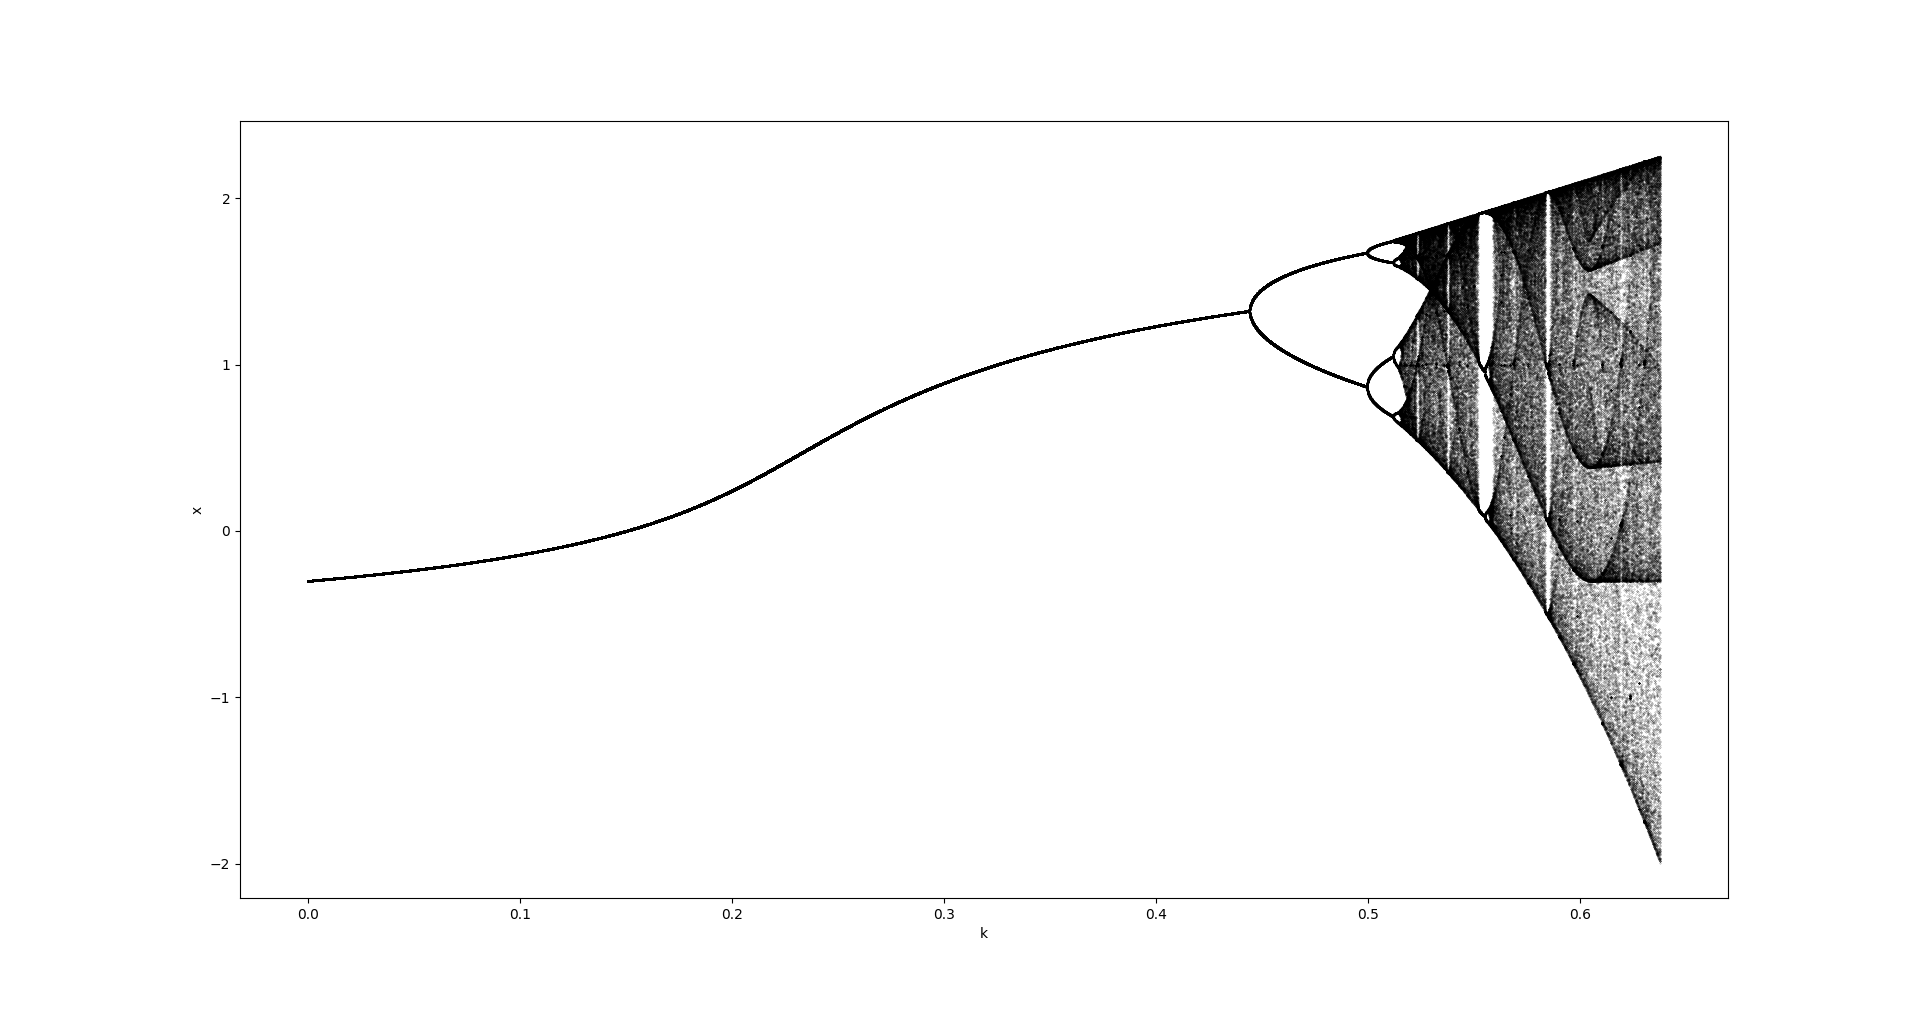
\includegraphics[width=1\linewidth]{LateX images/graphs q03/g1}
	\caption{ Διάγραμμα διακλάδωσης, για $q=-0.3$.}
	\label{f:g8}
\end{figure}

\begin{figure}[ht]
	\centering
	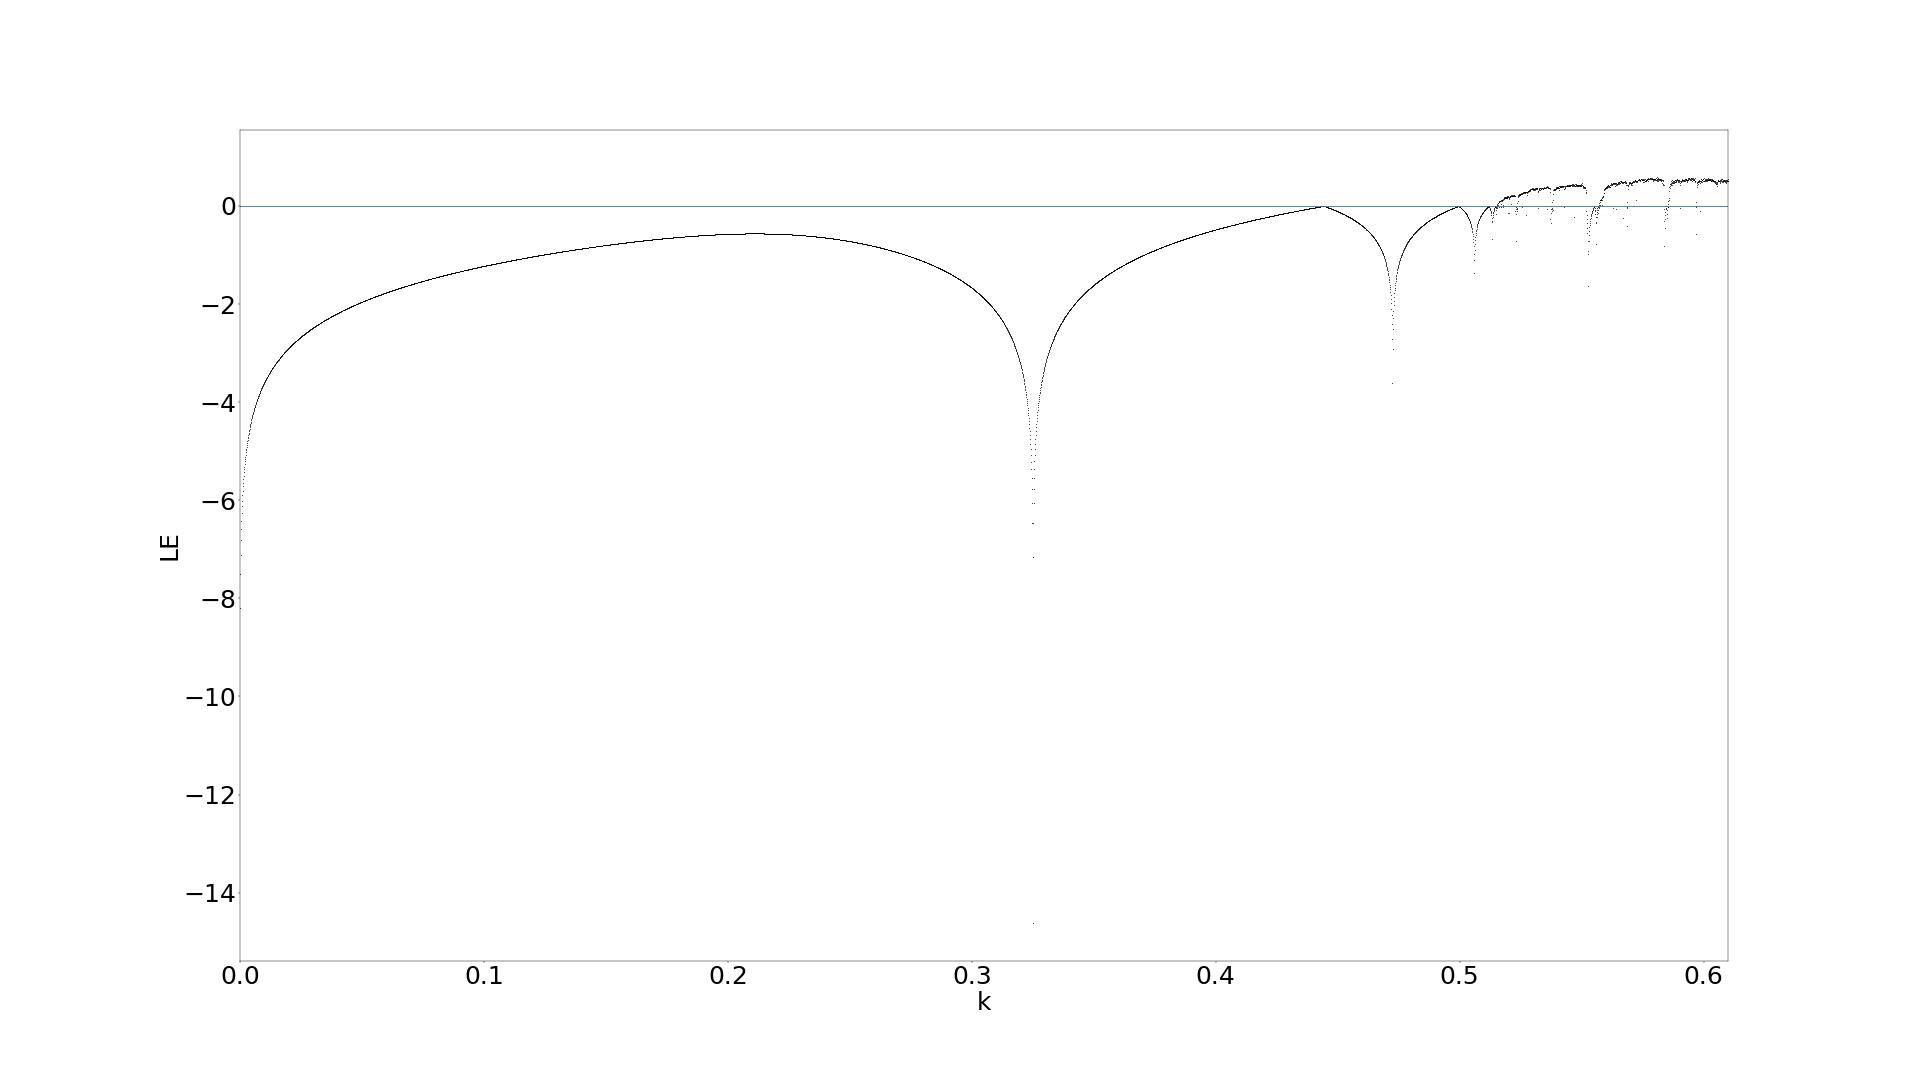
\includegraphics[width=1\linewidth]{LateX images/graphs q03/g2}
	\caption{ Διάγραμμα των εκθετών Lyapunov σε συνάρτηση με την παράμετρο \emph{k}, για $q=-0.3$.}
	\label{f:g9}
\end{figure}

\begin{figure}[ht]
	\centering	
	\begin{subfigure}[b]{0.4\textwidth}
		\centering
		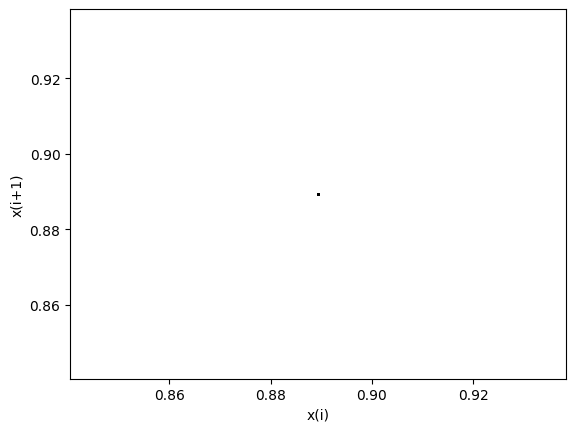
\includegraphics[width=\textwidth]{LateX images/graphs q03/g3}
		\caption{Για $k=0.3$}
		\label{f:k15}
	\end{subfigure}
	\hfill
	\begin{subfigure}[b]{0.4\textwidth}
		\centering
		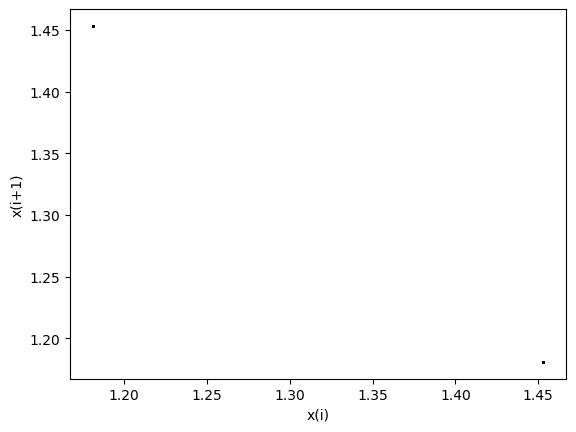
\includegraphics[width=\textwidth]{LateX images/graphs q03/g4}
		\caption{Για $k=0.44$}
		\label{f:k16}
	\end{subfigure}
	\hfill
	\begin{subfigure}[b]{0.4\textwidth}
		\centering
		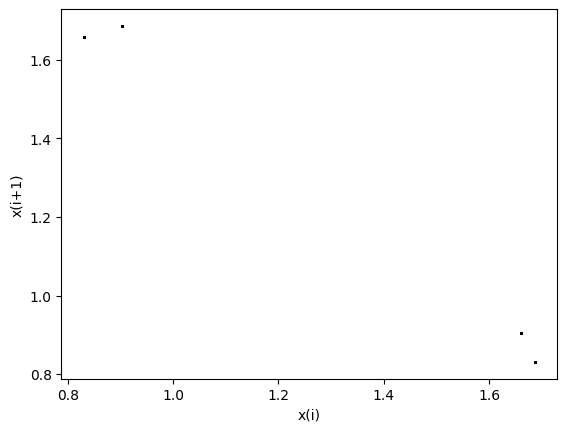
\includegraphics[width=\textwidth]{LateX images/graphs q03/g5}
		\caption{Για $k=0.5$}
		\label{f:k17}
	\end{subfigure}
	\hfill
	\begin{subfigure}[b]{0.4\textwidth}
		\centering
		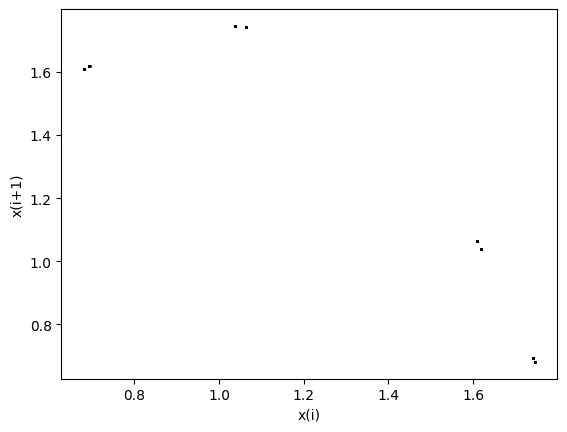
\includegraphics[width=\textwidth]{LateX images/graphs q03/g6}
		\caption{Για $k=0.511$}
		\label{f:k18}
	\end{subfigure}
	\hfill
	\begin{subfigure}[b]{0.4\textwidth}
		\centering
		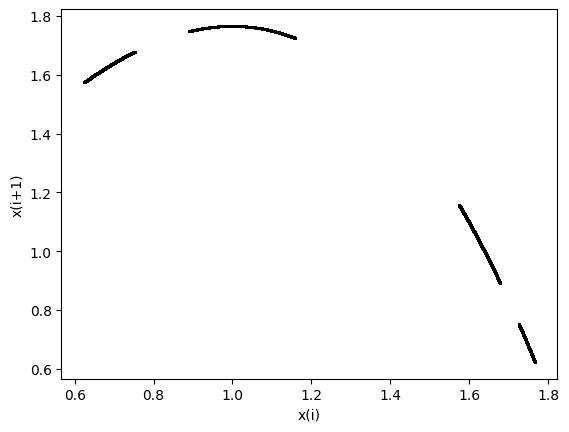
\includegraphics[width=\textwidth]{LateX images/graphs q03/g67}
		\caption{Για $k=0.5165$}
		\label{f:k19}
	\end{subfigure}
	\hfill
	\begin{subfigure}[b]{0.4\textwidth}
		\centering
		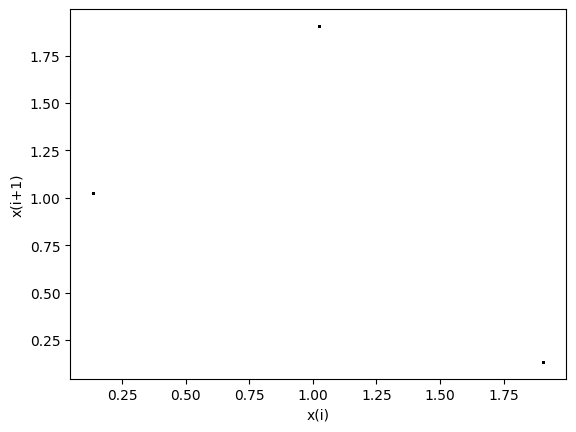
\includegraphics[width=\textwidth]{LateX images/graphs q03/g8}
		\caption{Για $k=0.551$}
		\label{f:k20}
	\end{subfigure}
	\hfill
	\caption{Διαγράμματα της τιμής \(x_i\) σε συνάρτηση με την τιμή \(x_{i+1}\) (α´μέρος).}	
\end{figure}
\begin{figure}[ht]
	\centering
	
	\begin{subfigure}[b]{0.4\textwidth}
		\centering
		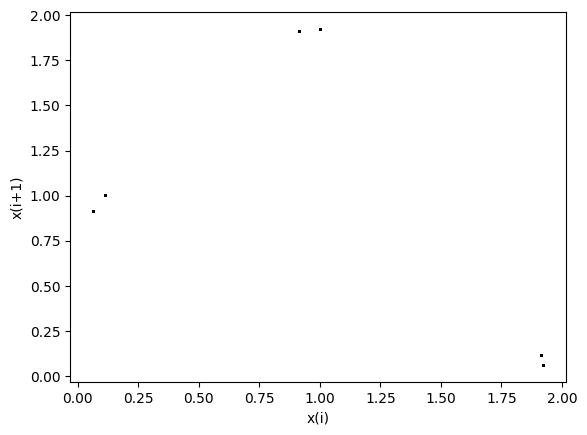
\includegraphics[width=\textwidth]{LateX images/graphs q03/g9}
		\caption{Για $k=0.555$}
		\label{f:k21}
	\end{subfigure}
	\hfill
	\begin{subfigure}[b]{0.4\textwidth}
		\centering
		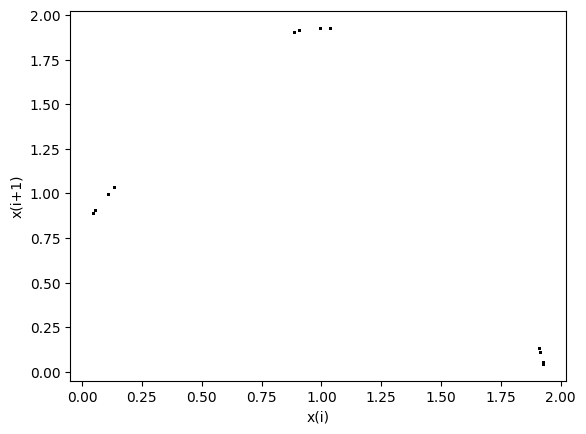
\includegraphics[width=\textwidth]{LateX images/graphs q03/g10}
		\caption{Για $k=0.556$}
		\label{f:k22}
	\end{subfigure}
	\hfill
	\begin{subfigure}[b]{0.4\textwidth}
		\centering
		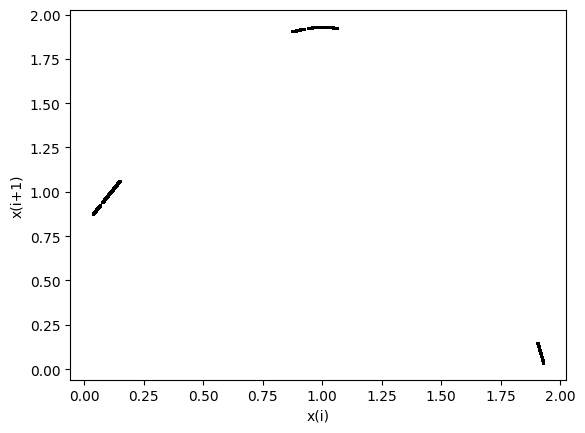
\includegraphics[width=\textwidth]{LateX images/graphs q03/g11}
		\caption{Για $k=0.5573$}
		\label{f:k23}
	\end{subfigure}
	\hfill
	\begin{subfigure}[b]{0.4\textwidth}
		\centering
		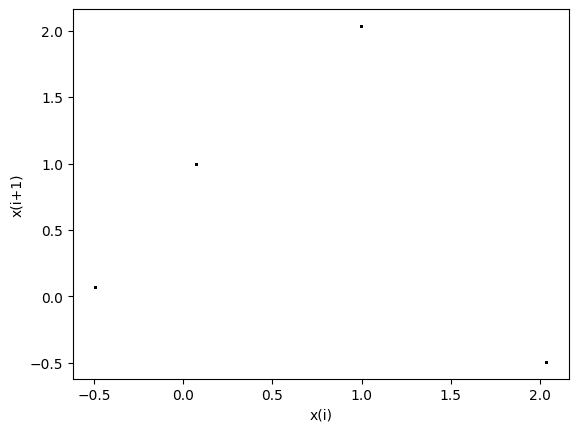
\includegraphics[width=\textwidth]{LateX images/graphs q03/g12}
		\caption{Για $k=0.583$}
		\label{f:k24}
	\end{subfigure}
	\hfill
	\begin{subfigure}[b]{0.4\textwidth}
		\centering
		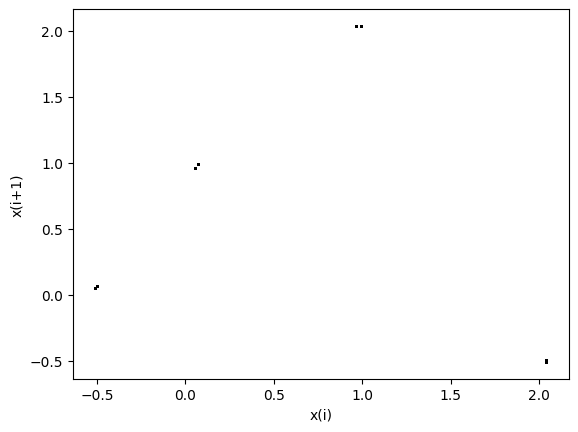
\includegraphics[width=\textwidth]{LateX images/graphs q03/g13}
		\caption{Για $k=0.5846$}
		\label{f:k25}
	\end{subfigure}
	\hfill
	\begin{subfigure}[b]{0.4\textwidth}
		\centering
		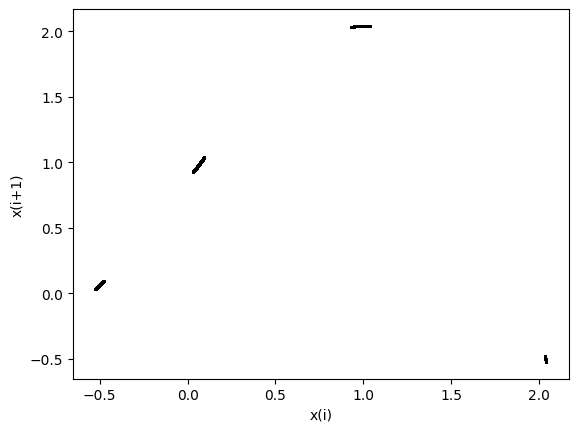
\includegraphics[width=\textwidth]{LateX images/graphs q03/g14}
		\caption{Για $k=0.5851$}
		\label{f:k26}
	\end{subfigure}
	\caption{Διαγράμματα της τιμής \(x_i\) σε συνάρτηση με την τιμή \(x_{i+1}\) (β´ μέρος).}	
\end{figure}

\clearpage

\section{Για q = -0.5}

Στο Σχ. \ref{f:g10} παρατίθεται το διάγραμμα διακλάδωσης του συστήματος \ref{f:x1}, ως προς την παράμετρο \emph{k}, για $q =- 0.5$. Για αυτές τις τιμές των παραμέτρων το σύστημα ξεκινάει από \emph{περίοδο - 1} για $k=0.3$, ενώ για  $k=0.48$ εμφανίζει τον πρώτο διπλασιασμό της περιόδου. Τον δεύτερο διπλασιασμό τον εμφανίζει για $k=0.53$ (\emph{περίοδος -   4}), τον τρίτο για $k=0.55$  (\emph{περίοδος -   8}) και τον τέταρτο για $k=0.5531$ (\emph{περίοδος -   16}). Στη συνέχεια για $k>0.5534$ το σύστημα εισέρχεται στο χάος, μέχρι να εξέλθει για $k=0.58$ (\emph{περίοδος -   3}) και να ξανά εισέλθει σε χάος μετά από δύο διπλασιασμούς $k=0.591$ (\emph{περίοδος -   6}), για $k>0.5927$.
Επομένως και σε αυτή την περίπτωση το σύστημα εισέρχεται στο χάος με διπλασιασμό της περιόδου. 

Επιπλέον, στο Σχ. \ref{f:g11} παρατίθεται το διάγραμμα των εκθετών Lyapunov για τιμές του \emph{k}, στο ίδιο διάστημα τιμών $[0, 0.679]$.  Στο διάστημα τιμών $0<k<0.5534$, στο $0.59<k<0.594$ παρατηρούμε ότι το διάγραμμα των εκθετών Lyapunov είναι συνεχώς αρνητικός, γεγονός που επιβεβαιώνει την περιοδική συμπεριφορά του συστήματος. Ενώ στα υπόλοιπα διαστήματα ο θετικός εκθέτης Lyapunov υποστηρίζει την χαοτική του συμπεριφορά, όπως έγινε φανερό και από το διάγραμμα διακλάδωσης.

Τέλος, στον πίνακα \ref{tab:abc2} παρατίθενται ενδεικτικές τιμές της παραμέτρου \emph{k} και η συμπεριφορά που παρουσιάζει το σύστημα για αυτές, σύμφωνα με το διάγραμμα διακλάδωσης, καθώς και τα αντίστοιχα σχήματα των διαγραμμάτων της τιμής \(x_i\) σε συνάρτηση με την τιμή \(x_{i+1}\). Από τα παραγόμενα σχήματα προκύπτει αριθμός σημείων αντίστοιχος με την περίοδο του συστήματος.\\\\

\begin{table}[ht]
	\centering
	\caption{ Συμπεριφορά του υπό μελέτη συστήματος για διάφορες τιμές του \emph{k}, για $q=-0.5$.}
	\label{tab:abc2}
	\begin{tabular}{l | l | l}
		Παράμετρος k & Συμπεριφορά & Σχήμα\\
		\hline
		0.3 &  Περίοδος - 1 & \ref{f:k27}\\
		0.48& Περίοδος - 2 & \ref{f:k28}\\
		0.53& Περίοδος - 4 & \ref{f:k29}\\
		0.55 &  Περίοδος - 8 & \ref{f:k30}\\
		0.5531 & Περίοδος - 16 & \ref{f:k31}\ \\
		0.5534 & Χάος & \ref{f:k32}\\
		0.58 & Περίοδος - 3 & \ref{f:k33})\\
		0.591 & Περίοδος - 6 & \ref{f:k35}\\
		0.5927 & Χάος & \ref{f:k36}\\
	\end{tabular}
	
\end{table}

\begin{figure}[ht]
	\centering
	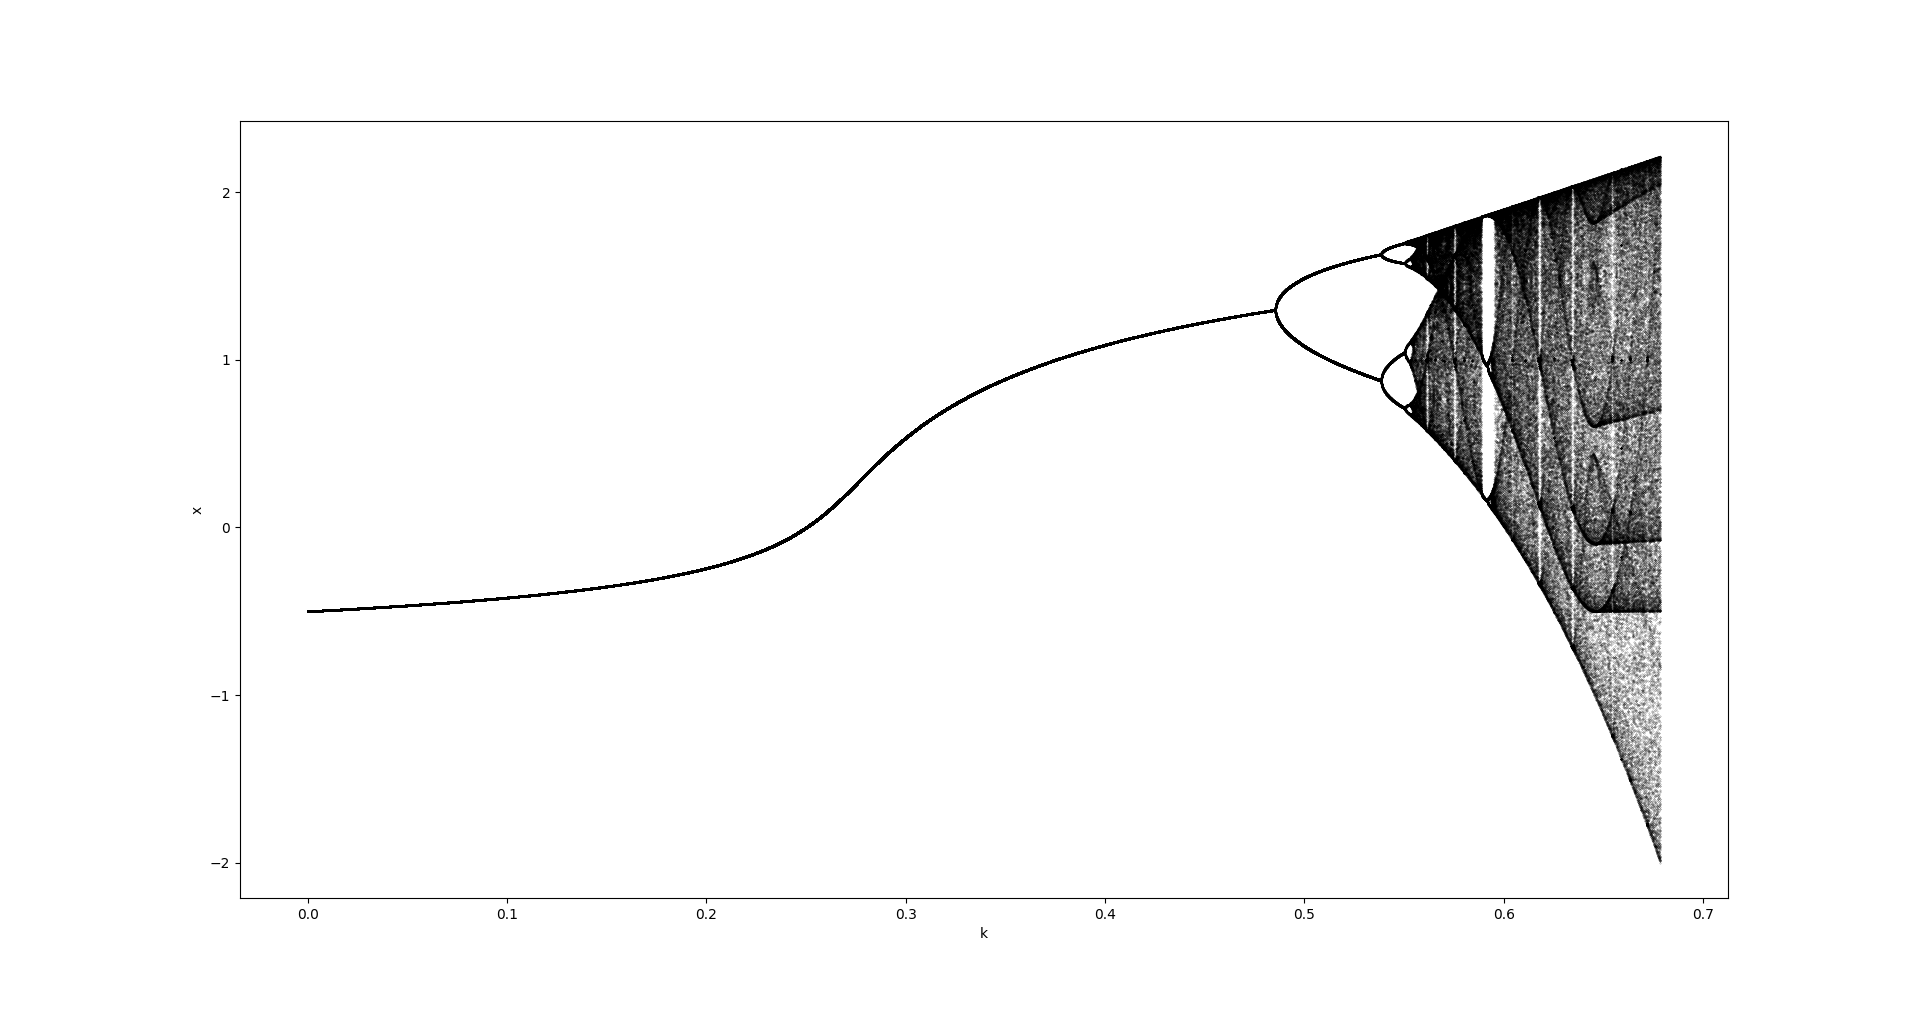
\includegraphics[width=1\linewidth]{LateX images/graphs q05/g1}
	\caption{ Διάγραμμα διακλάδωσης, για $q=-0.5$.}
	\label{f:g10}
\end{figure}

\begin{figure}[ht]
	\centering
	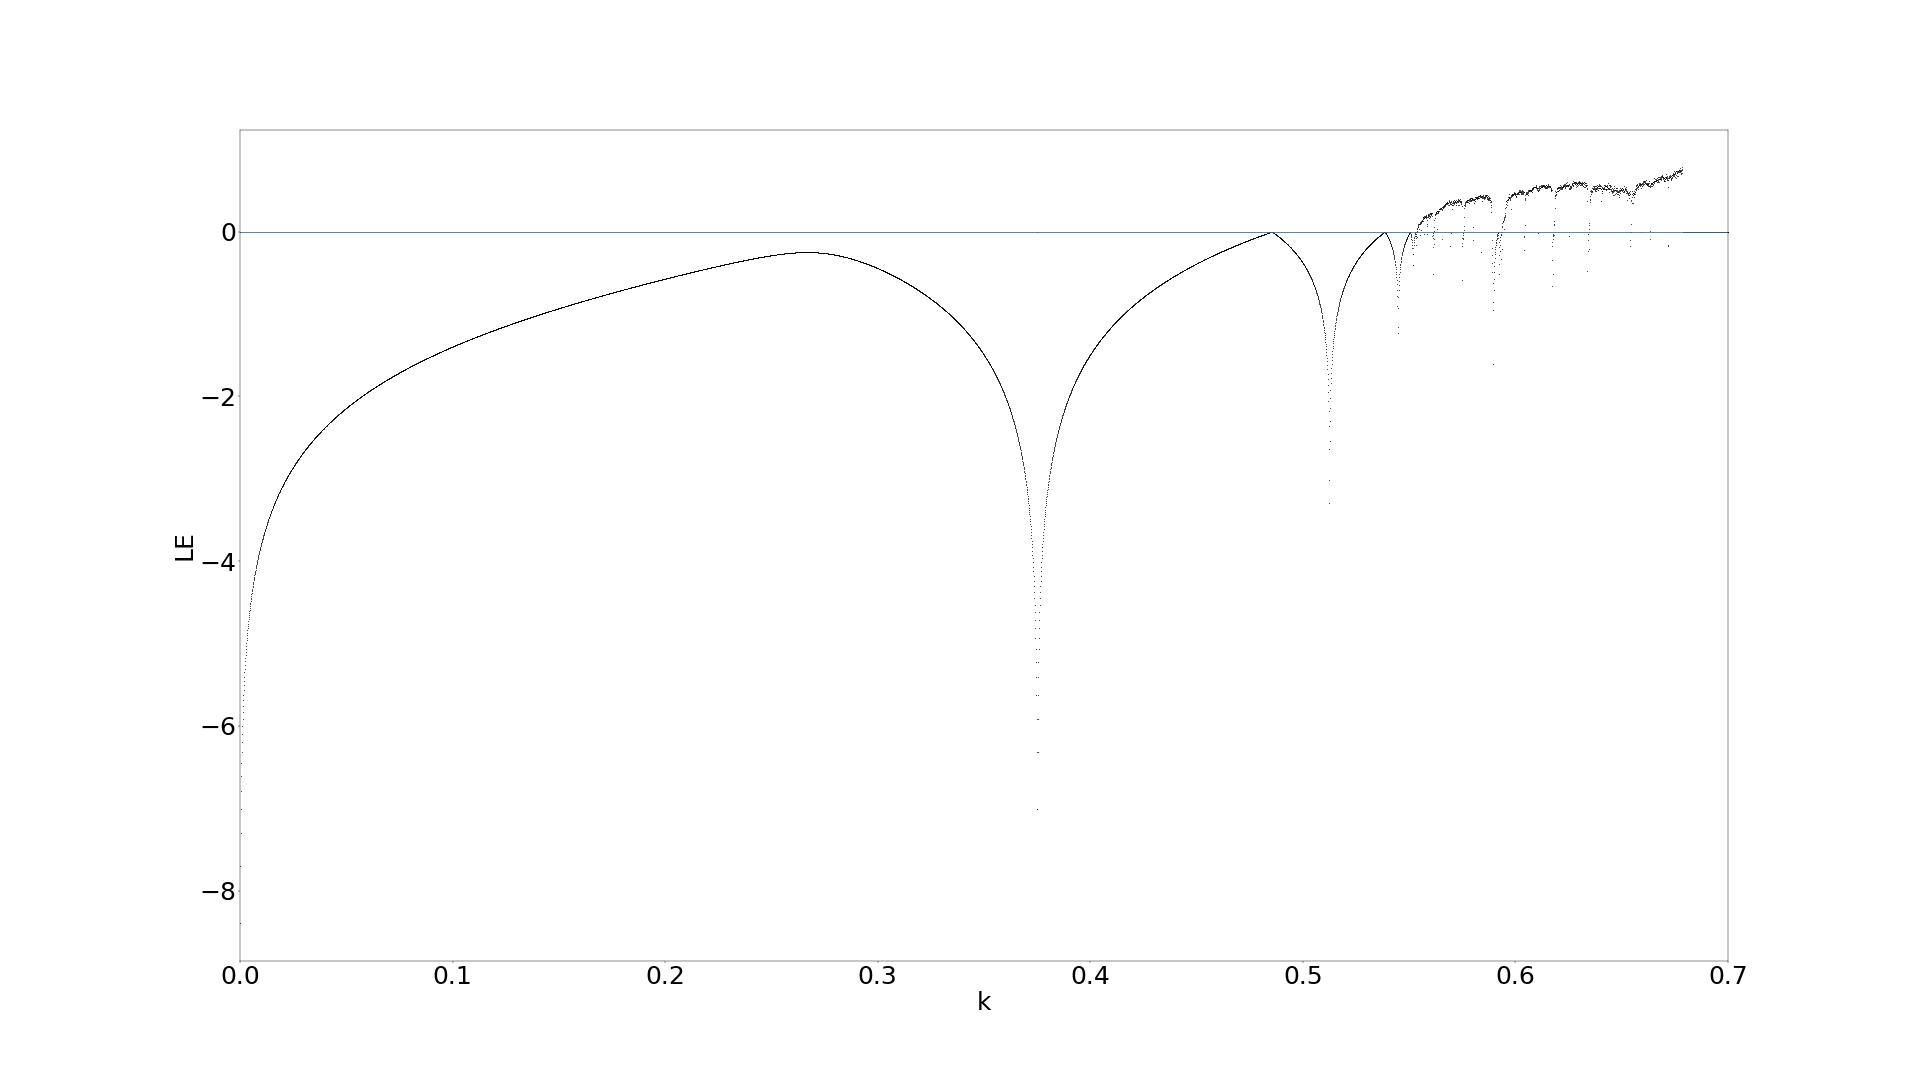
\includegraphics[width=1\linewidth]{LateX images/graphs q05/g2}
	\caption{ Διάγραμμα των εκθετών Lyapunov σε συνάρτηση με την παράμετρο \emph{k}, για $q=-0.5$.}
	\label{f:g11}
\end{figure}

\begin{figure}[ht]
	\centering
	\begin{subfigure}[b]{0.4\textwidth}
		\centering
		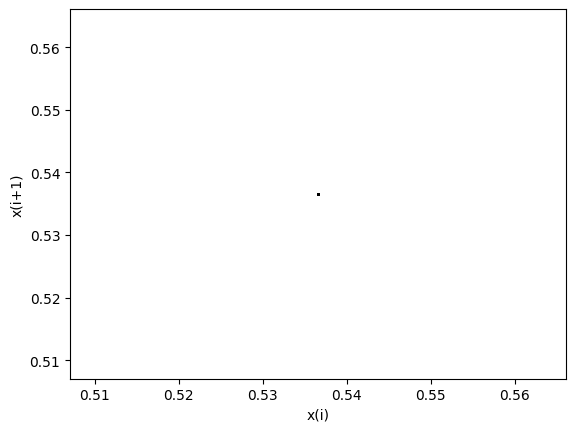
\includegraphics[width=\textwidth]{LateX images/graphs q05/g3}
		\caption{Για $k=0.3$}
		\label{f:k27}
	\end{subfigure}
	\hfill
	\begin{subfigure}[b]{0.4\textwidth}
		\centering
		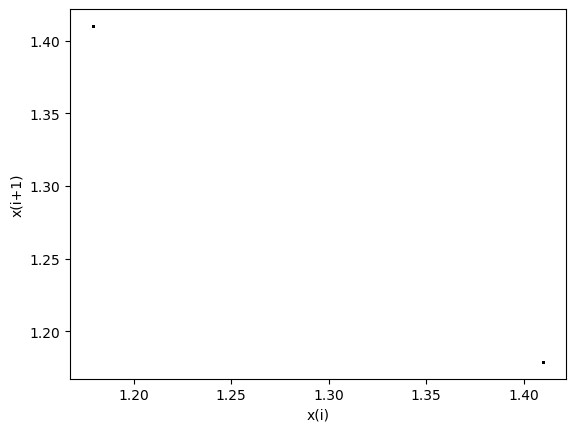
\includegraphics[width=\textwidth]{LateX images/graphs q05/g4}
		\caption{Για $k=0.48$}
		\label{f:k28}
	\end{subfigure}
	\hfill
	\begin{subfigure}[b]{0.4\textwidth}
		\centering
		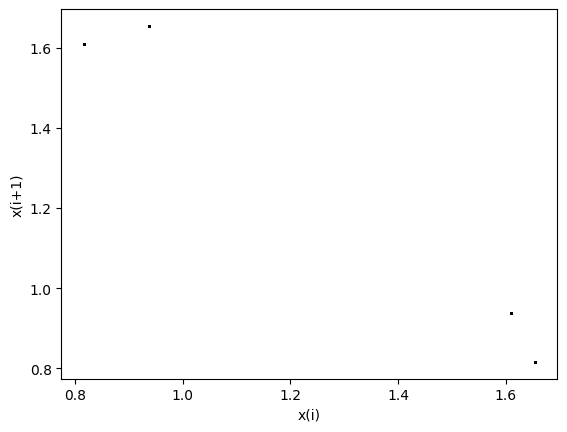
\includegraphics[width=\textwidth]{LateX images/graphs q05/g5}
		\caption{Για $k=0.53$}
		\label{f:k29}
	\end{subfigure}
	\hfill
	\begin{subfigure}[b]{0.4\textwidth}
		\centering
		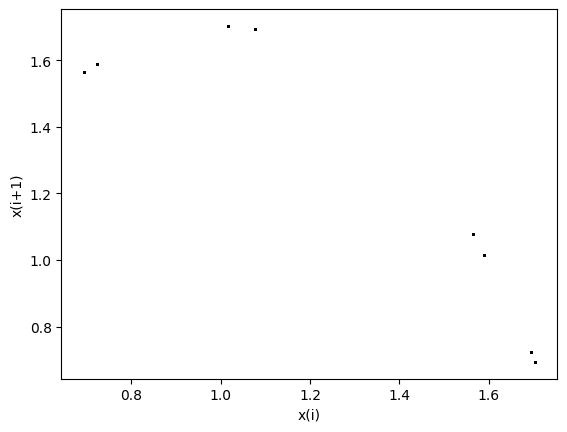
\includegraphics[width=\textwidth]{LateX images/graphs q05/g6}
		\caption{Για $k=0.55$}
		\label{f:k30}
	\end{subfigure}
	\hfill
	\caption{Διαγράμματα της τιμής \(x_i\) σε συνάρτηση με την τιμή \(x_{i+1}\) (α' μέρος).}
\end{figure}

\begin{figure}[ht]
	\begin{subfigure}[b]{0.4\textwidth}
		\centering
		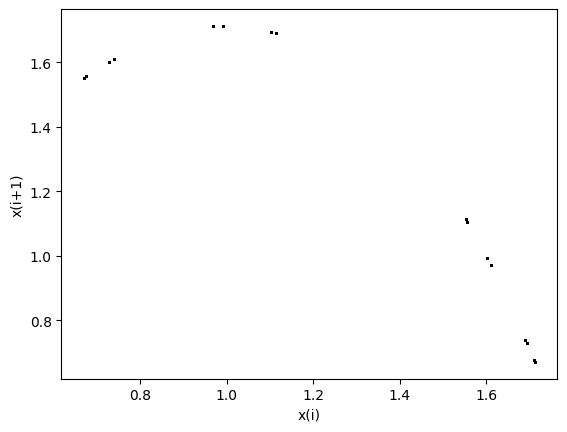
\includegraphics[width=\textwidth]{LateX images/graphs q05/g7}
		\caption{Για $k=0.5531$}
		\label{f:k31}
	\end{subfigure}
	\hfill
	\begin{subfigure}[b]{0.4\textwidth}
		\centering
		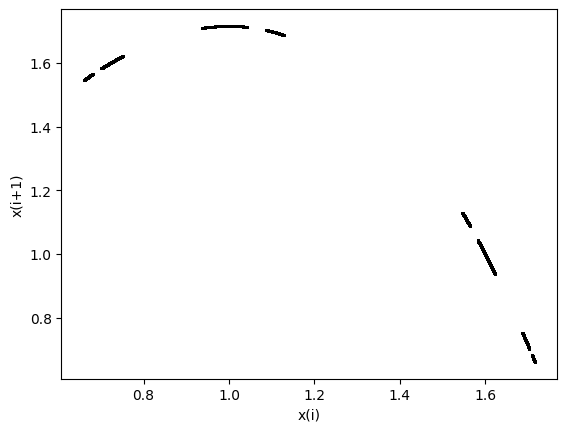
\includegraphics[width=\textwidth]{LateX images/graphs q05/g8}
		\caption{Για $k=0.5534$}
		\label{f:k32}
	\end{subfigure}
	\hfill
	\begin{subfigure}[c]{0.4\textwidth}
		\centering
		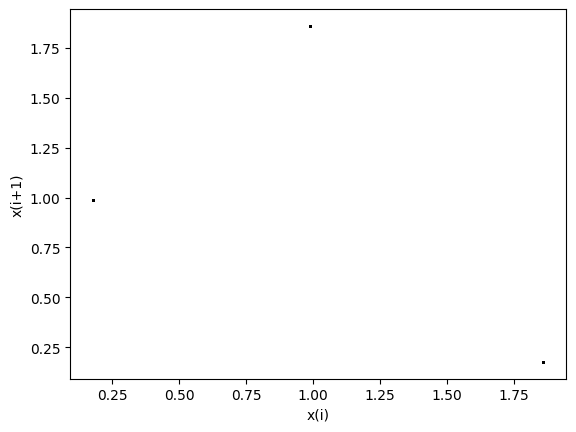
\includegraphics[width=\textwidth]{LateX images/graphs q05/g9}
		\caption{Για $k=0.58$}
		\label{f:k33}
	\end{subfigure}
	\hfill
	\begin{subfigure}[c]{0.4\textwidth}
		\centering
		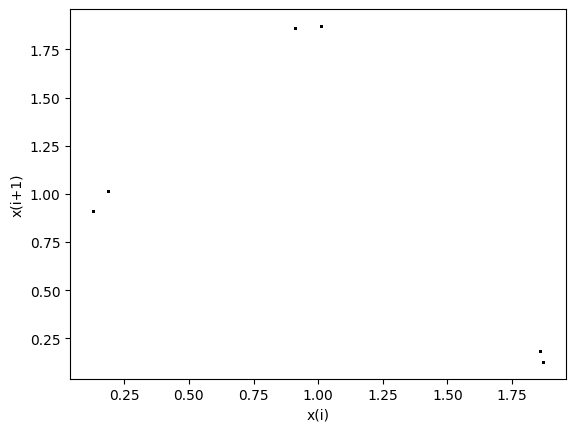
\includegraphics[width=\textwidth]{LateX images/graphs q05/g10}
		\caption{Για $k=0.591$}
		\label{f:k35}
	\end{subfigure}
	\hfill
	\centering
	\begin{subfigure}[b]{0.4\textwidth}
		\centering
		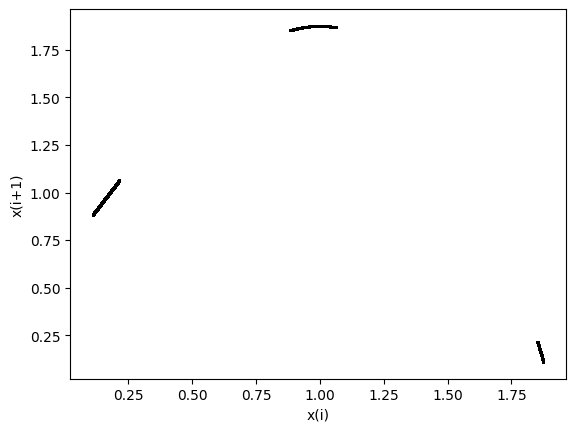
\includegraphics[width=\textwidth]{LateX images/graphs q05/g11}
		\caption{Για $k=0.5927$}
		\label{f:k36}
	\end{subfigure}
	\hfill
	\caption{Διαγράμματα της τιμής \(x_i\) σε συνάρτηση με την τιμή \(x_{i+1}\) (β´ μέρος).}		
\end{figure}

\clearpage

\section{Για q = -0.7}

Στο Σχ. \ref{f:g12} παρατίθεται το διάγραμμα διακλάδωσης του συστήματος \ref{f:x1}, ως προς την παράμετρο \emph{k}, για $q =- 0.7$. Για αυτές τις τιμές των παραμέτρων το σύστημα ξεκινάει από \emph{περίοδο - 1} για $k=0.3$ αλλά από $k[0.3469,0.3486]$ "σπάει" η περιοδική συμπεριφορά. Από $k=3.469$ το σύστημα εισέρχεται ξανά σε \emph{περίοδο - 1}. Για  $k = 0.52$ εμφανίζει τον πρώτο διπλασιασμό της περιόδου. Τον δεύτερο διπλασιασμό τον εμφανίζει για $k=0.57$  (\emph{περίοδος - 4}), τον τρίτο για $k=0.592$ (\emph{περίοδος - 8}) και τον τέταρτο για $k=0.593$ (\emph{περίοδος - 15}). Στη συνέχεια για $k>0.593$ το σύστημα εισέρχεται στο χάος, μέχρι να εξέλθει  για $k=0.627$ (\emph{περίοδος -   3}) και να ξανά εισέλθει σε χάος μετά από δύο διπλασιασμούς $k=0.63$  (\emph{περίοδος - 6}) $k=0.631$ (\emph{περίοδος -   11}), για $k>0.631$.
Επομένως και σε αυτή την περίπτωση το σύστημα εισέρχεται στο χάος με διπλασιασμό της περιόδου. 

Επιπλέον, στο Σχ. \ref{f:g11} παρατίθεται το διάγραμμα των εκθετών Lyapunov για τιμές του \emph{k} στο ίδιο διάστημα τιμών $[0, 0.72]$. Στο διάστημα τιμών $0<k<0.594$, στο $0.627<k<0.632$, παρατηρούμε ότι ο εκθέτης Lyapunov είναι συνεχώς αρνητικός, γεγονός που επιβεβαιώνει την περιοδική συμπεριφορά του συστήματος. Ενώ στα υπόλοιπα διαστήματα ο θετικός εκθέτης Lyapunov υποστηρίζει την χαοτική του συμπεριφορά, όπως έγινε φανερό και από το διάγραμμα διακλάδωσης.

Τέλος, στον πίνακα \ref{tab:abc3} παρατίθενται ενδεικτικές τιμές της παραμέτρου \emph{k} και η συμπεριφορά που παρουσιάζει το σύστημα για αυτές, σύμφωνα με το διάγραμμα διακλάδωσης, καθώς και τα αντίστοιχα σχήματα των διαγραμμάτων της τιμής \(x_i\) σε συνάρτηση με την τιμή \(x_{i+1}\). Από τα παραγόμενα σχήματα προκύπτει αριθμός σημείων αντίστοιχος με την περίοδο του συστήματος.\\\\

\begin{table}[ht]
	\centering
	\caption{ Συμπεριφορά του υπό μελέτη συστήματος για διάφορες τιμές του \emph{k}, για $q=-0.7$.}
	\label{tab:abc3}
	\begin{tabular}{l | l | l}
		Παράμετρος k & Συμπεριφορά & Σχήμα\\
		\hline
		0.25 &  Περίοδος -  1 & \ref{f:k37}\\
		0.3469&  Περίοδος -  1 & \ref{f:k38}\\
		0.52& Περίοδος -  2 & \ref{f:k39}\\
		0.57& Περίοδος -  4 & \ref{f:k40}\\
		0.592 &  Περίοδος -  8 & \ref{f:k41}\\
		0.593& Περίοδος -  15 & \ref{f:k42}\\
		0.594 & Χάος & \ref{f:k43}\\
		0.627 & Περίοδος -  3 & \ref{f:k44}\\
		0.630 & Περίοδος -  6 & \ref{f:k45}\\
		0.631 & Περίοδος -  11 & \ref{f:k46}\\
		0.632 & Χάος & \ref{f:k47}\\
	\end{tabular}
	
\end{table}

\begin{figure}[ht]
	\centering
	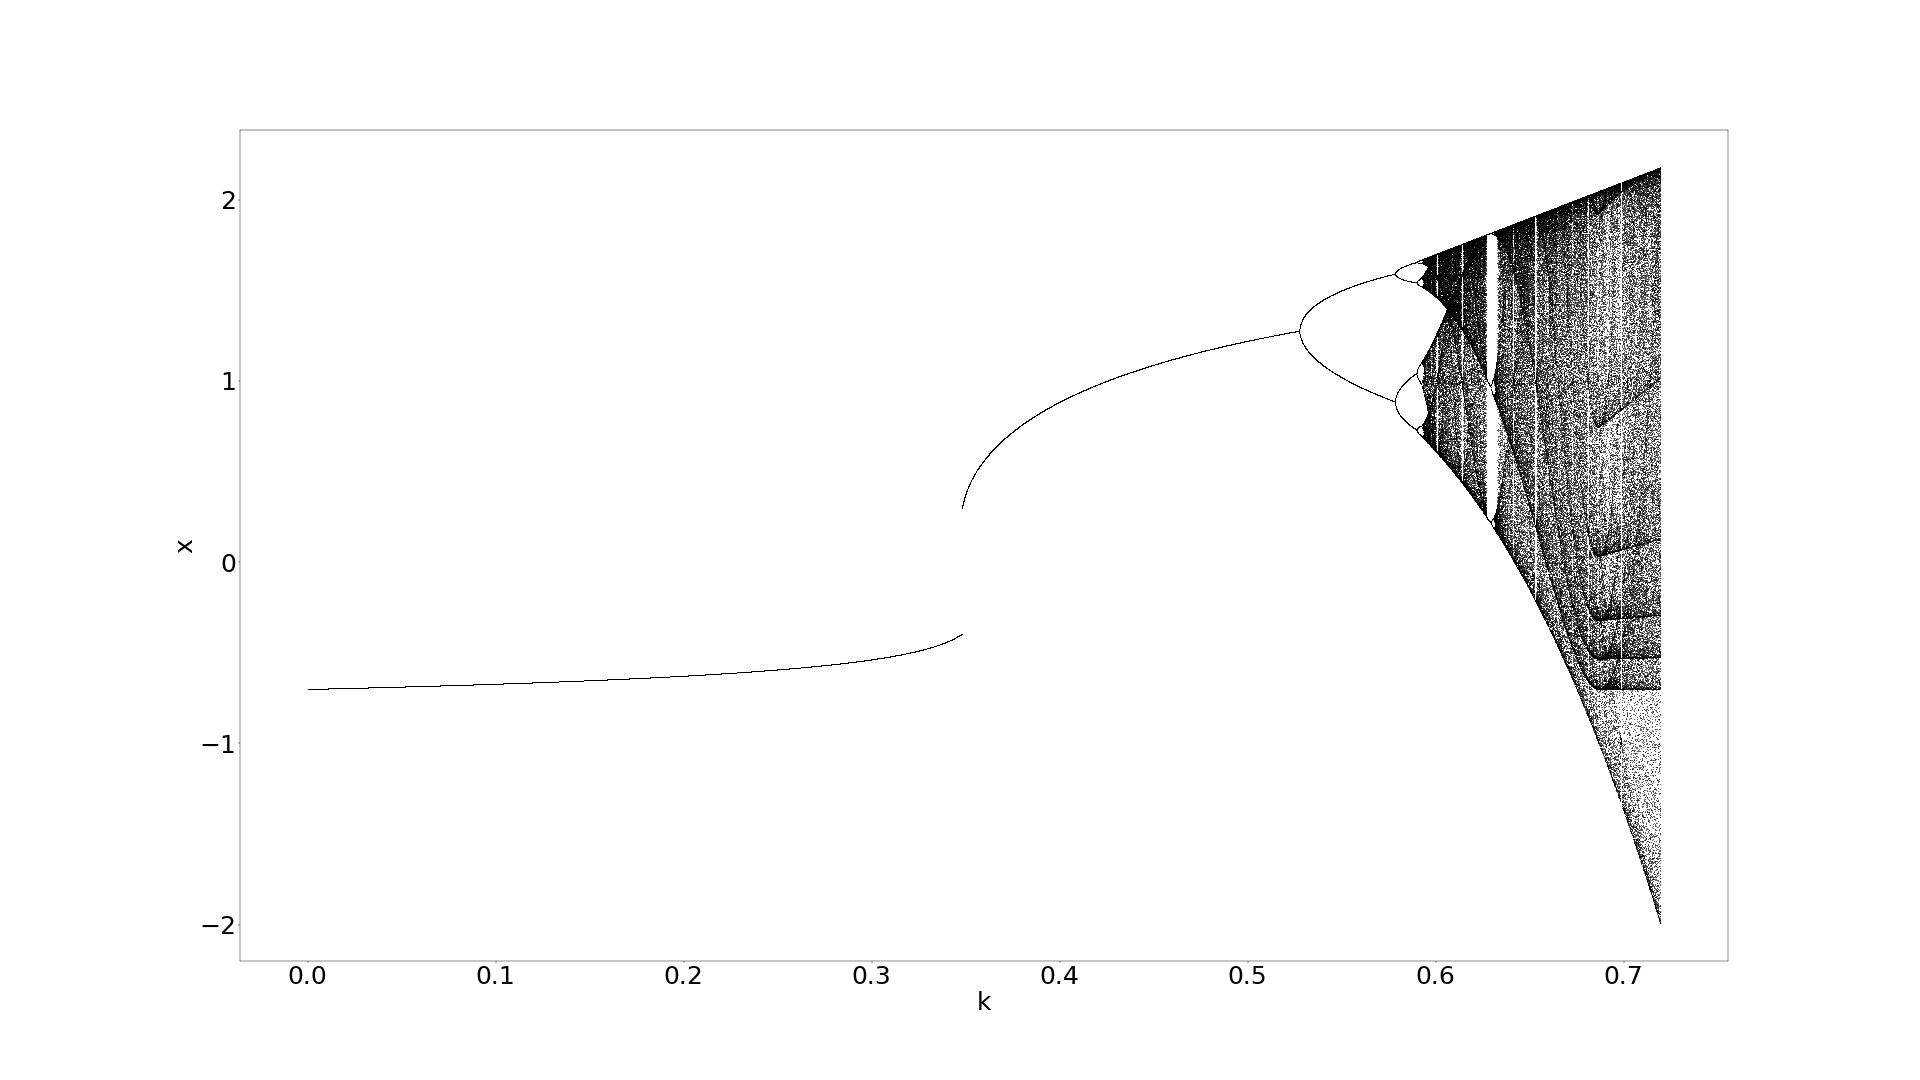
\includegraphics[width=1\linewidth]{LateX images/graphs q07/g1}
	\caption{ Διάγραμμα διακλάδωσης, για $q=-0.7$.}
	\label{f:g12}
\end{figure}
\begin{figure}[ht]
	\centering
	\includegraphics[width=1\linewidth]{"LateX images/graphs q07/g2 "}
	\caption{Διάγραμμα των εκθετών Lyapunov σε συνάρτηση με την παράμετρο \emph{k}, για $q=-0.7$.}
	\label{f:g13}
\end{figure}

\begin{figure}[ht]
	\centering
	
	\begin{subfigure}[b]{0.4\textwidth}
		\centering
		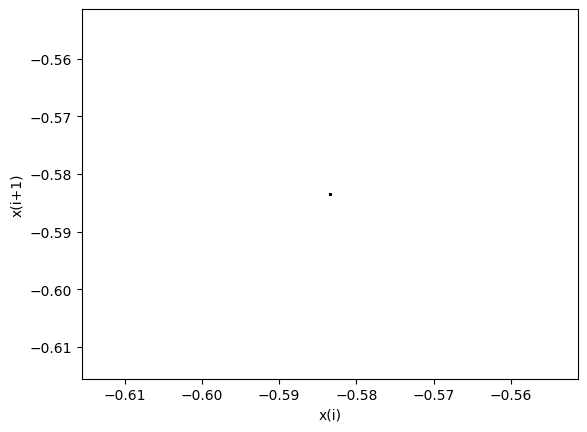
\includegraphics[width=\textwidth]{LateX images/graphs q07/g3}
		\caption{Για $k=0.25$}
		\label{f:k37}
	\end{subfigure}
	\hfill
	\begin{subfigure}[b]{0.4\textwidth}
		\centering
		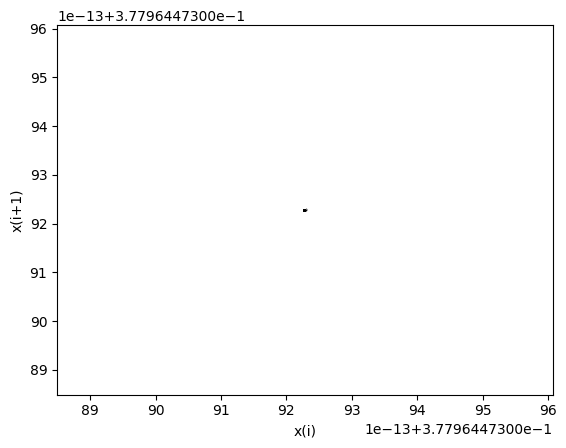
\includegraphics[width=\textwidth]{LateX images/graphs q07/g4}
		\caption{Για $k=0.3469$}
		\label{f:k38}
	\end{subfigure}
	\hfill
	\begin{subfigure}[b]{0.4\textwidth}
		\centering
		\includegraphics[width=\textwidth]{LateX images/graphs q07/g5}
		\caption{Για $k=0.52$}
		\label{f:k39}
	\end{subfigure}
	\hfill
	\begin{subfigure}[b]{0.4\textwidth}
		\centering
		\includegraphics[width=\textwidth]{LateX images/graphs q07/g6}
		\caption{Για $k=0.57$}
		\label{f:k40}
	\end{subfigure}
	\hfill
	\begin{subfigure}[b]{0.4\textwidth}
		\centering
		\includegraphics[width=\textwidth]{LateX images/graphs q07/g7}
		\caption{Για $k=0.592$}
		\label{f:k41}
	\end{subfigure}
	\hfill
	\caption{Διαγράμματα της τιμής \(x_i\) σε συνάρτηση με την τιμή \(x_{i+1}\) (α' μέρος).}
\end{figure}

\begin{figure}[ht]
	\centering
	\begin{subfigure}[b]{0.4\textwidth}
		\centering
		\includegraphics[width=\textwidth]{LateX images/graphs q07/g8}
		\caption{χια $k=0.593$}
		\label{f:k42}
	\end{subfigure}
	\hfill
	\begin{subfigure}[b]{0.4\textwidth}
		\centering
		\includegraphics[width=\textwidth]{LateX images/graphs q07/g9}
		\caption{Για $k=0.594$}
		\label{f:k43}
	\end{subfigure}
	\hfill
	\begin{subfigure}[b]{0.4\textwidth}
		\centering
		\includegraphics[width=\textwidth]{LateX images/graphs q07/g10}
		\caption{Για $k=0.627$}
		\label{f:k44}
	\end{subfigure}
	\hfill
	\begin{subfigure}[b]{0.4\textwidth}
		\centering
		\includegraphics[width=\textwidth]{LateX images/graphs q07/g11}
		\caption{Για $k=0.63$}
		\label{f:k45}
	\end{subfigure}
	\hfill
	\begin{subfigure}[b]{0.4\textwidth}
		\centering
		\includegraphics[width=\textwidth]{LateX images/graphs q07/g12}
		\caption{Για $k=0.631$}
		\label{f:k46}
	\end{subfigure}
	\hfill
	\begin{subfigure}[b]{0.4\textwidth}
		\centering
		\includegraphics[width=\textwidth]{LateX images/graphs q07/g13}
		\caption{Για $k=0.632$}
		\label{f:k47}
	\end{subfigure}
	\caption{Διαγράμματα της τιμής \(x_i\) σε συνάρτηση με την τιμή \(x_{i+1}\) (β' μέρος).}	
\end{figure}

\clearpage

\section{Για q = -0.9}

Στο Σχ. \ref{f:g14} παρατίθεται το διάγραμμα διακλάδωσης του συστήματος \ref{f:x1}, ως προς την παράμετρο \emph{k}, για $q =- 0.9$. Για αυτές τις τιμές των παραμέτρων το σύστημα ξεκινάει από \emph{περίοδο - 1} για $k=0.3$ αλλά στο διάστημα τιμών $0.43<k<0.436$ "σπάει" η περιοδική συμπεριφορά. Οπότε το σύστημα εμφανίζει πάλι το φαινόμενο της υστέρησης. Απο $k=3.436$ το σύστημα εμφανίζει πάλι περιοδική συμπεριφορά \emph{περίοδο - 1}. Για  $k = 0.57$ εμφανίζει τον πρώτο διπλασιασμό της περιόδου. Τον δεύτερο διπλασιασμό τον εμφανίζει για $k=0.62$ (\emph{περίοδος - 4}), τον τρίτο για $k=0.63$ (\emph{περίοδος - 8}) και τον τέταρτο για $k=0.633$ (\emph{περίοδος - 16}). Στην συνέχεια για $k>0.635$ το σύστημα εισέρχεται στο χάος, μέχρι να εξέλθει για $k=0.665$ (\emph{περίοδος - 3}) και να ξανά εισέλθει στο χάος μετά από έναν νέο διπλασιασμό $k=0.668$ (\emph{περίοδος - 6)}, για $k>0.671$. Παρόλα αυτά παρατηρείται μία ακόμα έξοδος από το χάος για $k=0.72$ (\emph{περίοδος - 1}).Για $q=-0.7$ το σύστημα εισέρχεται στο χάος με διπλασιασμό της περιόδου.

Επιπλέον, στο σχήμα \ref{f:g15} παρατίθεται το διάγραμμα των εκθετών Lyapunov για τιμές του \emph{k} στο ίδιο διάστημα τιμών $[0, 0.77]$. Στο διάστημα τιμών   $0<k<0.635$, στο $0.665<k<0.671$ και $0.72<k<0.77$ παρατηρούμε ότι ο εκθέτης Lyapunov είναι συνεχώς αρνητικός, γεγονός που επιβεβαιώνει την περιοδική συμπεριφορά του συστήματος. Ενώ στα υπόλοιπα διαστήματα ο θετικός εκθέτης Lyapunov υποστηρίζει τη χαοτική του συμπεριφορά, όπως έγινε φανερό και από το διάγραμμα διακλάδωσης.

Τέλος, στον πίνακα \ref{tab:abc4} παρατίθενται ενδεικτικές τιμές της παραμέτρου \emph{k} και η συμπεριφορά που παρουσιάζει το σύστημα για αυτές, σύμφωνα με το διάγραμμα διακλάδωσης, καθώς και τα αντίστοιχα σχήματα των διαγραμμάτων της τιμής \(x_i\) σε συνάρτηση με την τιμή \(x_{i+1}\). Από τα παραγόμενα σχήματα προκύπτει αριθμός σημείων αντίστοιχος με την περίοδο του συστήματος.\\\\

\begin{table}[ht]
	\centering
	\caption{ Συμπεριφορά του υπό μελέτη συστήματος για διάφορες τιμές του \emph{k}, για $q=-0.9$.}
	\label{tab:abc4}
	\begin{tabular}{l | l | l}
		Παράμετρος k & Συμπεριφορά & Σχήμα\\
		\hline
		0.43 &  Περίοδος -  1 & \ref{f:k48}\\
		0.436 &  Περίοδος -  1 & \ref{f:k49}\\
		0.57& Περίοδος -  2 & \ref{f:k50}\\
		0.62& Περίοδος -  4 & \ref{f:k51}\\
		0.63 &  Περίοδος -  8 & \ref{f:k52}\\
		0.633& Περίοδος -  16 & \ref{f:k53}\\
		0.635& Χάος & \ref{f:k54}\\
		0.665 & Περίοδος -  3 & \ref{f:k55}\\
		0.668 & Περίοδος -  6 & \ref{f:k56}\\
		0.671 & Χάος & \ref{f:k57}\\
		0.72 & Περίοδος -  1& \ref{f:k58}\\
	\end{tabular}
\end{table}

\begin{figure}[ht]
	\centering
	\includegraphics[width=1\linewidth]{LateX images/graphs q09/g1}
	\caption{ Διάγραμμα διακλάδωσης, για $q=-0.7$.}
	\label{f:g14}
\end{figure}

\begin{figure}[ht]
	\centering
	\includegraphics[width=1\linewidth]{LateX images/graphs q09/g2}
	\caption{Διάγραμμα των εκθετών Lyapunov σε συνάρτηση με την παράμετρο \emph{k}, για $q=-0.7$}
	\label{f:g15}
\end{figure}

\begin{figure}[ht]
	\centering
	\begin{subfigure}[b]{0.4\textwidth}
		\centering
		\includegraphics[width=\textwidth]{LateX images/graphs q09/g3}
		\caption{Για $k=0.43$}
		\label{f:k48}
	\end{subfigure}
	\hfill
	\begin{subfigure}[b]{0.4\textwidth}
		\centering
		\includegraphics[width=\textwidth]{LateX images/graphs q09/g4}
		\caption{Για $k=0.436$}
		\label{f:k49}
	\end{subfigure}
	\hfill
	\begin{subfigure}[b]{0.4\textwidth}
		\centering
		\includegraphics[width=\textwidth]{LateX images/graphs q09/g5}
		\caption{Για $k=0.57$}
		\label{f:k50}
	\end{subfigure}
	\hfill
	\begin{subfigure}[b]{0.4\textwidth}
		\centering
		\includegraphics[width=\textwidth]{LateX images/graphs q09/g6}
		\caption{Για $k=0.62$}
		\label{f:k51}
	\end{subfigure}
	\hfill
	\begin{subfigure}[b]{0.4\textwidth}
		\centering
		\includegraphics[width=\textwidth]{LateX images/graphs q09/g13}
		\caption{Για $k=0.63$}
		\label{f:k52}
	\end{subfigure}
	\hfill
	\caption{Διαγράμματα της τιμής \(x_i\) σε συνάρτηση με την τιμή \(x_{i+1}\) (α' μέρος).}
\end{figure}
\begin{figure}
	\centering
	\begin{subfigure}[b]{0.4\textwidth}
		\centering
		\includegraphics[width=\textwidth]{LateX images/graphs q09/g7}
		\caption{Για $k=0.633$}
		\label{f:k53}
	\end{subfigure}
	\hfill
	\begin{subfigure}[b]{0.4\textwidth}
		\centering
		\includegraphics[width=\textwidth]{LateX images/graphs q09/g8}
		\caption{Για $k=0.635$}
		\label{f:k54}
	\end{subfigure}
	\hfill
	\begin{subfigure}[b]{0.4\textwidth}
		\centering
		\includegraphics[width=\textwidth]{LateX images/graphs q09/g9}
		\caption{Για $k=0.665$}
		\label{f:k55}
	\end{subfigure}
	\hfill
	\begin{subfigure}[b]{0.4\textwidth}
		\centering
		\includegraphics[width=\textwidth]{LateX images/graphs q09/g10}
		\caption{Για $k=0.668$}
		\label{f:k56}
	\end{subfigure}
	\hfill
	\begin{subfigure}[b]{0.4\textwidth}
		\centering
		\includegraphics[width=\textwidth]{LateX images/graphs q09/g11}
		\caption{Για $k=0.671$}
		\label{f:k57}
	\end{subfigure}
	\hfill
	\begin{subfigure}[b]{0.4\textwidth}
		\centering
		\includegraphics[width=\textwidth]{LateX images/graphs q09/g12}
		\caption{Για $k=0.72$}
		\label{f:k58}
	\end{subfigure}
	\hfill
	\caption{Διαγράμματα της τιμής \(x_i\) σε συνάρτηση με την τιμή \(x_{i+1}\) (β' μέρος).}
\end{figure}

\clearpage

\section{Για q = -1.2}
Στο Σχ. \ref{f:g16} παρατίθεται το διάγραμμα διακλάδωσης του συστήματος \ref{f:x1}, ως προς την παράμετρο \emph{k}, για $q =- 1.2$. Για αυτές τις τιμές των παραμέτρων το σύστημα ξεκινάει από \emph{περίοδο - 1} για $k = 0.55$, αλλά στο διάστημα τιμών $0.56<k<0.566$ "σπάει" η περιοδική συμπεριφορά, εμφανιζοντας το φαινόμενο της υστέρησης. Από $k=0.566$ το σύστημα εμφανίζει πάλι περιοδική συμπεριφορά \emph{περίοδο - 1}. Για  $k = 0.63$ εμφανίζει τον πρώτο διπλασιασμό της περιόδου. Τον δεύτερο διπλασιασμό τον εμφανίζει για $k=0.67$ (\emph{περίοδος - 4}) και τον τρίτο για $k=0.69$ (\emph{περίοδος -   8}). Στη συνέχεια για $k>0.696$ το σύστημα εισέρχεται στο χάος, μέχρι να εξέλθει για $k=0.726$  (\emph{περίοδος - 3}) και να ξανά εισέλθει στο χάος μετά από ένα διπλασιασμό $k=0.729$ (\emph{περίοδος - 6}), για $k>0.731$. Παρόλα αυτά παρατηρείται μία ακόμα έξοδος από το χάος για $k=0.762$ (\emph{περίοδος -   1}). Για $q=-1.2$το σύστημα εισέρχεται στο χάος με διπλασιασμό της περιόδου, ενώ παρατηρείται και εσωτερική κρίση ελκυστή για $k=0.726$ αλλά και για $k=0.762$.

Επιπλέον, στο Σχ. \ref{f:g17} παρατίθεται το διάγραμμα των εκθετών Lyapunov για τιμές του \emph{k} στο ίδιο διάστημα τιμών $[0, 0.77]$. Στο διάστημα τιμών  $0<k<0.69$, στο $0.726<k<0.731$ και στο $0.72<k<0.8574$ παρατηρούμε ότι ο εκθέτης Lyapunov είναι συνεχώς αρνητικός, γεγονός που επιβεβαιώνει την περιοδική συμπεριφορά του συστήματος. Ενώ στα υπόλοιπα διαστήματα ο θετικός εκθέτης Lyapunov υποστηρίζει την χαοτική του συμπεριφορά, όπως έγινε φανερό και από το διάγραμμα διακλάδωσης.

Τέλος, στον πίνακα \ref{tab:abc5} παρατίθενται ενδεικτικές τιμές της παραμέτρου \emph{k} και η συμπεριφορά που παρουσιάζει το σύστημα για αυτές, σύμφωνα με το διάγραμμα διακλάδωσης, καθώς και τα αντίστοιχα σχήματα των διαγραμμάτων της τιμής \(x_i\) σε συνάρτηση με την τιμή \(x_{i+1}\). Από τα παραγόμενα σχήματα προκύπτει αριθμός σημείων αντίστοιχος με την περίοδο του συστήματος.\\\\

\begin{table}[ht]
	\centering
	\caption{ Συμπεριφορά του υπό μελέτη συστήματος για διάφορες τιμές του \emph{k}, για $q=-1.2$.}
	\label{tab:abc5}
	\begin{tabular}{l | l | l}
		Παράμετρος k & Συμπεριφορά & Σχήμα\\
		\hline
		0.55 &  Περίοδος -  1 & \ref{f:k59}\\
		0.566 &  Περίοδος -  1 & \ref{f:k60}\\
		0.63& Περίοδος -  2 & \ref{f:k61}\\
		0.68& Περίοδος -  4 & \ref{f:k62}\\
		0.69 &  Περίοδος -  8 & \ref{f:k63}\\
		0.696& Χάος & \ref{f:k64}\\
		0.726& Περίοδος -  3 & \ref{f:k65}\\
		0.729& Περίοδος -  6 & \ref{f:k66}\\
		0.731& Χάος & \ref{f:k67}\\
		0.762 &  Περίοδος -  1 & \ref{f:k68}\\
	\end{tabular}
\end{table}

\begin{figure}[ht]
	\centering
	\includegraphics[width=1\linewidth]{LateX images/graphs q12/g1}
	\caption{ Διάγραμμα διακλάδωσης, για $q=-1.2$.}
	\label{f:g16}
\end{figure}

\begin{figure}[ht]
	\centering
	\includegraphics[width=1\linewidth]{LateX images/graphs q12/g2}
	\caption{Διάγραμμα των εκθετών Lyapunov σε συνάρτηση με την παράμετρο \emph{k}, για $q=-1.2$.}
	\label{f:g17}
\end{figure}

\begin{figure}[ht]
	\centering
	
	\begin{subfigure}[b]{0.4\textwidth}
		\centering
		\includegraphics[width=\textwidth]{LateX images/graphs q12/g3}
		\caption{Για $k=0.55$}
		\label{f:k59}
	\end{subfigure}
	\hfill
	\begin{subfigure}[b]{0.4\textwidth}
		\centering
		\includegraphics[width=\textwidth]{LateX images/graphs q12/g4}
		\caption{Για $k=0.566$}
		\label{f:k60}
	\end{subfigure}
	\hfill
	\begin{subfigure}[b]{0.4\textwidth}
		\centering
		\includegraphics[width=\textwidth]{LateX images/graphs q12/g5}
		\caption{Για $k=0.63$}
		\label{f:k61}
	\end{subfigure}
	\hfill
	\begin{subfigure}[b]{0.4\textwidth}
		\centering
		\includegraphics[width=\textwidth]{LateX images/graphs q12/g6}
		\caption{Για $k=0.68$}
		\label{f:k62}
	\end{subfigure}
	\hfill
	\begin{subfigure}[b]{0.4\textwidth}
		\centering
		\includegraphics[width=\textwidth]{LateX images/graphs q12/g7}
		\caption{Για $k=0.69$}
		\label{f:k63}
	\end{subfigure}
	\hfill
	\begin{subfigure}[b]{0.4\textwidth}
		\centering
		\includegraphics[width=\textwidth]{LateX images/graphs q12/g8}
		\caption{Για $k=0.696$}
		\label{f:k64}
	\end{subfigure}
	\hfill
	\caption{Διαγράμματα της τιμής \(x_i\) σε συνάρτηση με την τιμή \(x_{i+1}\) (α' μέρος).}
\end{figure}
\begin{figure}[ht]
	\centering
	\begin{subfigure}[b]{0.4\textwidth}
		\centering
		\includegraphics[width=\textwidth]{LateX images/graphs q12/g9}
		\caption{Για $k=0.726$}
		\label{f:k65}
	\end{subfigure}
	\hfill
	\begin{subfigure}[b]{0.4\textwidth}
		\centering
		\includegraphics[width=\textwidth]{LateX images/graphs q12/g10}
		\caption{Για $k=0.729$}
		\label{f:k66}
	\end{subfigure}
	\hfill
	\begin{subfigure}[b]{0.4\textwidth}
		\centering
		\includegraphics[width=\textwidth]{LateX images/graphs q12/g11}
		\caption{Για $k=0.731$}
		\label{f:k67}
	\end{subfigure}
	\hfill
	\begin{subfigure}[b]{0.4\textwidth}
		\centering
		\includegraphics[width=\textwidth]{LateX images/graphs q12/g12}
		\caption{Για $k=0.762$}
		\label{f:k68}
	\end{subfigure}
	\hfill
	\caption{Διαγράμματα της τιμής \(x_i\) σε συνάρτηση με την τιμή \(x_{i+1}\) (β' μέρος).}	
\end{figure}

\clearpage

\section{Για q = -1.4}
Στα Σχ. \ref{f:20} , \ref{f:21} παρατίθενται τα διαγράμματα διακλάδωσης του συστήματος \ref{f:x1}, ως προς την παράμετρο \emph{k}, για $a = 1$, $b = 2$ , $q =- 1.4$ και για διαφορετικές αρχικές συνθήκες δηλαδή για διαφορετικό \(x_0\). Συγκρίνοντας το διάγραμμα \ref{f:g19} (\(x_0=0.1\)) με τα υπόλοιπα διαγράμματα διακλάδωσης \ref{f:g20} (\(x_0=0.5\)), \ref{f:g21} (\(x_0=1\)), \ref{f:g22} (\(x_0=-0.1\)) παρατηρείται ότι για $q=-1.4$ εμφανίζεται το φαινόμενο της συνύπαρξης ελκυστών. Η συμπεριφορά του συστήματος για τις διάφορες περιπτώσεις επιβεβαιώνεται και από τα αντίστοιχα διαγράμματα Lyapunov \ref{f:g23}, \ref{f:g24}, \ref{f:g25}, \ref{f:g26},
όπως και απο το διάγραμμα διακλάδωσης \ref{f:g231}, όπου η κάθε αρχική συνθήκη εμφανίζεται με διαφορετικό χρώμα.

Στον πίνακα \ref{tab:abc6} φαίνεται η πορεία του συστήματος και για ποιες τιμές της παραμέτρου \emph{k} το σύστημα εμφανίζει περιοδική ή χαοτική συμπεριφορά, σύμφωνα με το διάγραμμα διακλάδωσης \ref{f:g19}. Οι τιμές αυτές αντιστοιχούν στα σχήματα των διαγραμμάτων της τιμής \(x_i\) σε συνάρτηση με την τιμή \(x_{i+1}\). Από τα παραγόμενα σχήματα προκύπτει αριθμός σημείων αντίστοιχος με την περίοδο του συστήματος.

Επίσης παρατηρείται η εσωτερική κρίση ελκυστών για διάφορες τιμές του \emph{k} (0.744, 0.7565 , 0.768 , 0.8), όπως και το φαινόμενο της υστέρησης το οποίο φαίνεται στο διάγραμμα διακλάδωσης \ref{f:g19} στην μεταπήδηση του συστήματος από χαοτική συμπεριφορά σε περίοδο-2, αλλά και από \emph{περίοδο - 2} σε \emph{περίοδο - 1}. Οι αντίστοιχες τιμές του \emph{k} για αυτά τα σημεία του διαγράμματος υπάρχουν στο πίνακα \ref{tab:abc7}.

Τέλος, στο σχήμα \ref{f:g23} παρατίθεται το διάγραμμα των εκθετών Lyapunov για τιμές του \emph{k} στο ίδιο διάστημα τιμών $[0, 0.91]$. Οι τιμές του πίνακα \ref{tab:abc6} που έχουνε περιοδική συμπεριφορά αντιστοιχούν σε τιμές του διαγράμματος \ref{f:g23} όπου ο εκθέτης Lyapunov είναι συνεχώς αρνητικός, γεγονός που επιβεβαιώνει την συμπεριφορά τους. Ενώ για τις υπόλοιπες τιμές ο θετικός εκθέτης Lyapunov υποστηρίζει την χαοτική τους συμπεριφορά, όπως έγινε φανερό και από το διάγραμμα διακλάδωσης.

\begin{table}[ht]
	\centering
	\caption{ Συμπεριφορά του υπό μελέτη συστήματος για διάφορες τιμές του \emph{k}, για $a = 1$, $b = 2$ , $q=-1.4$ και
		\(x_i=0.1\)}
	\label{tab:abc6}
	\begin{tabular}{l | l | l}
		Παράμετρος k & Συμπεριφορά & Σχήμα\\
		\hline
		0.4 &  Περίοδος -  1 & \ref{f:k}\\
		0.54 &  Περίοδος -  2 & \ref{f:k69}\\
		0.65& Περίοδος -  1 & \ref{f:k70}\\
		0.68& Περίοδος -  2 & \ref{f:k71}\\
		0.726 &  Περίοδος -  4 & \ref{f:k72}\\
		0.737& Περίοδος -  8 & \ref{f:k73}\\
		0.738& Περίοδος -  15 & \ref{f:k74}\\
		0.739& Χάος & \ref{f:k75}\\
		0.744 &  Περίοδος -  6 & \ref{f:k76}\\
		0.746 &  Χάος & \ref{f:k77}\\
		0.7565 &  Περίοδος -  5 & \ref{f:k78}\\
		0.757 &  Χάος & \ref{f:k79}\\
		0.768 &  Περίοδος -  3 & \ref{f:k83}\\
		0.77 &  Περίοδος -  6 & \ref{f:k80}\\
		0.78 &  Χάος & \ref{f:k81}\\
		0.8 & Περίοδος -  2&\ref{f:k82}\\
	\end{tabular}
\end{table}

\begin{figure}[ht]
	\centering
	
	\begin{subfigure}[b]{1\textwidth}
		\centering
		\includegraphics[width=\textwidth]{LateX images/graphs q14/g1}
		\caption{\(x_0=0.1\)}
		\label{f:g19}
	\end{subfigure}
	\hfill
	\begin{subfigure}[b]{1\textwidth}
		\centering
		\includegraphics[width=\textwidth]{LateX images/graphs q14/g2}
		\caption{\(x_0=0.5\)}
		\label{f:g20}
	\end{subfigure}
	\hfill
	
	\caption{ Διαγράμματα διακλάδωσης, για $q=-1.4$ (α' μέρος).}
	\label{f:20}
\end{figure}
\begin{figure}
	\centering
	\begin{subfigure}[b]{1\textwidth}
		\centering
		\includegraphics[width=\textwidth]{LateX images/graphs q14/g3}
		\caption{\(x_0=1\)}
		\label{f:g21}
	\end{subfigure}
	\hfill
	\begin{subfigure}[b]{1\textwidth}
		\centering
		\includegraphics[width=\textwidth]{LateX images/graphs q14/g4}
		\caption{\(x_0=-0.1\)}
		\label{f:g22}
	\end{subfigure}
	\hfill
	\caption{ Διαγράμματα διακλάδωσης, για $q=-1.4$ (β' μέρος).}
	\label{f:21}
\end{figure}

\begin{figure}[ht]
	\centering
	
	\begin{subfigure}[b]{1\textwidth}
		\centering
		\includegraphics[width=\textwidth]{LateX images/graphs q14/g6}
		\caption{Για \(x_0=0.1\)}
		\label{f:g23}
	\end{subfigure}
	\hfill
	\begin{subfigure}[b]{1\textwidth}
		\centering
		\includegraphics[width=\textwidth]{LateX images/graphs q14/g7}
		\caption{Για \(x_0=0.5\)}
		\label{f:g24}
	\end{subfigure}
	\hfill
	\caption{ Διαγράμματα των εκθετών Lyapunov σε συνάρτηση με την παράμετρο \emph{k}, για  $q=-1.4$ (α' μέρος). }
\label{f:g233}
\end{figure}

\begin{figure}[ht]
	\centering

	\begin{subfigure}[b]{1\textwidth}
		\centering
		\includegraphics[width=\textwidth]{LateX images/graphs q14/g8}
		\caption{Για \(x_0=1\)}
		\label{f:g25}
	\end{subfigure}
	\hfill
	\begin{subfigure}[b]{1\textwidth}
		\centering
		\includegraphics[width=\textwidth]{LateX images/graphs q14/g9}
		\caption{ΓΙα \(x_0=-0.1\)}
		\label{f:g26}
	\end{subfigure}
	\hfill
	\caption{ Διαγράμματα των εκθετών Lyapunov σε συνάρτηση με την παράμετρο \emph{k}, για  $q=-1.4$ (β' μέρος).}
	\label{f:g2333}
\end{figure}

\begin{figure}[ht]
	\centering
	\includegraphics[width=1\linewidth]{LateX images/graphs q14/g30}
	\caption{Διάγραμμα διακλάδωσης, για όλες τις διαφορετικές αρχικές συνθήκες $x_0$}
	\label{f:g231}
\end{figure}

\begin{figure}[ht]
	\centering
	
	\begin{subfigure}[b]{0.4\textwidth}
		\centering
		\includegraphics[width=\textwidth]{LateX images/graphs q14/g11}
		\caption{Για $k=0.4$}
		\label{f:k}
	\end{subfigure}
	\hfill
	\begin{subfigure}[b]{0.4\textwidth}
		\centering
		\includegraphics[width=\textwidth]{LateX images/graphs q14/g12}
		\caption{Για $k=0.54$}
		\label{f:k69}
	\end{subfigure}
	\hfill
	\begin{subfigure}[b]{0.4\textwidth}
		\centering
		\includegraphics[width=\textwidth]{LateX images/graphs q14/g13}
		\caption{Για $k=0.65$}
		\label{f:k70}
	\end{subfigure}
	\hfill
	\begin{subfigure}[b]{0.4\textwidth}
		\centering
		\includegraphics[width=\textwidth]{LateX images/graphs q14/g14}
		\caption{Για $k=0.68$}
		\label{f:k71}
	\end{subfigure}
	\hfill
	\begin{subfigure}[b]{0.4\textwidth}
		\centering
		\includegraphics[width=\textwidth]{LateX images/graphs q14/g15}
		\caption{Για $k=0.726$}
		\label{f:k72}
	\end{subfigure}
	\hfill
	\begin{subfigure}[b]{0.4\textwidth}
		\centering
		\includegraphics[width=\textwidth]{LateX images/graphs q14/g16}
		\caption{Για $k=0.737$}
		\label{f:k73}
	\end{subfigure}
	\hfill
	\caption{Διαγράμματα της τιμής \(x_i\) σε συνάρτηση με την τιμή \(x_{i+1}\) (α' μέρος).}
\end{figure}
\begin{figure}[ht]
	\centering
	\begin{subfigure}[b]{0.4\textwidth}
		\centering
		\includegraphics[width=\textwidth]{LateX images/graphs q14/g17}
		\caption{Για $k=0.738$}
		\label{f:k74}
	\end{subfigure}
	\hfill
	\begin{subfigure}[b]{0.4\textwidth}
		\centering
		\includegraphics[width=\textwidth]{LateX images/graphs q14/g18}
		\caption{Για $k=0.739$}
		\label{f:k75}
	\end{subfigure}
	\hfill
	\begin{subfigure}[b]{0.4\textwidth}
		\centering
		\includegraphics[width=\textwidth]{LateX images/graphs q14/g19}
		\caption{Για $k=0.744$}
		\label{f:k76}
	\end{subfigure}
	\hfill
	\begin{subfigure}[b]{0.4\textwidth}
		\centering
		\includegraphics[width=\textwidth]{LateX images/graphs q14/g20}
		\caption{Για $k=0.746$}
		\label{f:k77}
	\end{subfigure}
	\hfill
	\begin{subfigure}[b]{0.4\textwidth}
		\centering
		\includegraphics[width=\textwidth]{LateX images/graphs q14/g21}
		\caption{Για $k=0.7565$}
		\label{f:k78}
	\end{subfigure}
	\hfill
	\begin{subfigure}[b]{0.4\textwidth}
		\centering
		\includegraphics[width=\textwidth]{LateX images/graphs q14/g22}
		\caption{Για $k=0.757$}
		\label{f:k79}
	\end{subfigure}
	\hfill	
	\begin{subfigure}[b]{0.4\textwidth}
		\centering
		\includegraphics[width=\textwidth]{LateX images/graphs q14/g23}
		\caption{Για $k=0.768$}
		\label{f:k83}
	\end{subfigure}
	\hfill
	\begin{subfigure}[b]{0.4\textwidth}
		\centering
		\includegraphics[width=\textwidth]{LateX images/graphs q14/g24}
		\caption{Για $k=0.77$}
		\label{f:k80}
	\end{subfigure}
	\hfill
	\caption{Διαγράμματα της τιμής \(x_i\) σε συνάρτηση με την τιμή \(x_{i+1}\) (β' μέρος).}
\end{figure}

\begin{figure}[ht]
	\centering
	\begin{subfigure}[b]{0.4\textwidth}
		\centering
		\includegraphics[width=\textwidth]{LateX images/graphs q14/g25}
		\caption{Για $k=0.78$.}
		\label{f:k81}
	\end{subfigure}
	\hfill
	\begin{subfigure}[b]{0.4\textwidth}
		\centering
		\includegraphics[width=\textwidth]{LateX images/graphs q14/g26}
		\caption{Για $k=0.8$.}
		\label{f:k82}
	\end{subfigure}
	\hfill	
	\caption{Διαγράμματα της τιμής \(x_i\) σε συνάρτηση με την τιμή \(x_{i+1}\) (γ' μέρος).}	
\end{figure}

\clearpage
\section{Για q = -1.6}
%%%%%%%%%%%%%%%
%ΓΙΑ ΑΥΤΟ το συστημα οταν μεταπηδα απο χαος σε χαος Θεωρείται υστέρηση
%%%%%%%%%%%%%%%%%%%%%
Στα Σχ. \ref{f:g234}, \ref{f:g235}  παρατίθενται τα διαγράμματα διακλάδωσης του συστήματος \ref{f:x1}, ως προς την παράμετρο \emph{k}, για  $q =- 1.6$ και για διαφορετικές αρχικές συνθήκες, δηλαδή για διαφορετικό \(x_0\). Συγκρίνοντας το διάγραμμα \ref{f:g27} (\(x_0=0.1\)) με τα υπόλοιπα διαγράμματα διακλάδωσης \ref{f:g28}  (\(x_0=0.5\)), \ref{f:g29}  (\(x_0=1\)), \ref{f:g30}  (\(x_0=1.5\)), \ref{f:g31}  (\(x_0=2\)), \ref{f:g32}  (\(x_0=-0.1\)) παρατηρείται ότι για $q= -1.6$ εμφανίζεται το φαινόμενο της συνύπαρξης ελκυστών. Η συμπεριφορά του συστήματος για τις διάφορες περιπτώσεις επιβεβαιώνεται και από τα διαγράμματα Lyapunov \ref{f:g33}, \ref{f:g34}, \ref{f:g35}, \ref{f:g36}, \ref{f:g37}, \ref{f:g38} , όπως και απο το διάγραμμα διακλάδωσης \ref{f:g232}, όπου η κάθε αρχική συνθήκη εμφανίζεται με διαφορετικό χρώμα.

Στο διάγραμμα διακλάδωσης \ref{f:g27} εμφανίζονται κάποιες διακοπές της γραφικής παράστασης στην περιοχή του χάους. Αυτό οφείλεται στο ότι η δυναμική συμπεριφορά του συστήματος αποκλίνει σε πολύ μεγάλες τιμές.

Στον πίνακα \ref{tab:abc7} φαίνεται η πορεία του συστήματος και για ποιες τιμές της παραμέτρου  \emph{k} το σύστημα εμφανίζει περιοδική ή χαοτική συμπεριφορά, σύμφωνα με το διάγραμμα διακλάδωσης \ref{f:g27}.

Επίσης παρατηρείται εσωτερική κρίση ελκυστών για διάφορες τιμές του \emph{k} (0.683, 0.7, 0.715, 0.74, 0.788, 0.799, 0.81, 0.94), όπως και το φαινόμενο της υστέρησης το οποίο φαίνεται στο διάγραμμα διακλάδωσης \ref{f:g27} στα κενά μεταξύ χάους και περιοδικής συμπεριφοράς, όπως και στην μεταπήδηση του συστήματος από χαοτική συμπεριφορά σε περίοδο-2. Οι αντίστοιχες τιμές του \emph{k} για αυτά τα σημεία του διαγράμματος υπάρχουν στο πίνακα \ref{tab:abc7},όπως και τα αντίστοιχα σχήματα των διαγραμμάτων της τιμής \(x_i\) σε συνάρτηση με την τιμή \(x_{i+1}\). Από τα παραγόμενα σχήματα προκύπτει αριθμός σημείων αντίστοιχος με την περίοδο του συστήματος.

Τέλος, στο σχήμα \ref{f:g31} παρατίθεται το διάγραμμα των εκθετών Lyapunov για τιμές του \emph{k} στο ίδιο διάστημα τιμών $[0, 0.982]$. Οι τιμές του πίνακα \ref{tab:abc7} που έχουνε περιοδική συμπεριφορά αντιστοιχούν σε τιμές του διαγράμματος \ref{f:g27} όπου ο εκθέτης Lyapunov είναι συνεχώς αρνητικός, γεγονός που επιβεβαιώνει την συμπεριφορά τους. Ενώ για τις υπόλοιπες τιμές ο θετικός εκθέτης Lyapunov υποστηρίζει την χαοτική τους συμπεριφορά, όπως έγινε φανερό και από το διάγραμμα διακλάδωσης.\\\\


\begin{table}[ht]
	\centering
	\caption{ Συμπεριφορά του υπό μελέτη συστήματος για διάφορες τιμές του \emph{k}, για $q=-1.6$, για \(x_i=0.1\)}
	\label{tab:abc7}
	\begin{tabular}{l | l }
		Παράμετρος k & Συμπεριφορά \\
		\hline
		0.31 &  Περίοδος -  1 \\
		0.34 &  Περίοδος -  2 \\
		0.595& Περίοδος -  4 \\
		0.66& Περίοδος -  8 \\
		0.671 &  Περίοδος -  12\\
		0.675& Χαός \\
		0.683& Περίοδος -  12 \\
		0.685& Χάος \\
		0.7 &  Περίοδος -  18\\
		0.71&  Χάος \\
		0.715 &  Περίοδος -  6\\
		0.716 &  Περίοδος -  12\\
		0.717 &  Χάος \\
		0.74 & Περίοδος -  2\\
		0.77 &  Περίοδος -  4 \\
		0.779 &  Περίοδος -  8\\
		0.782 & Χάος\\
		0.788 & Περίοδος -  20\\
		0.789 & Χάος\\
		0.799 & Περίοδος -  5\\
		0.8 &Χάος\\
		0.81 & Περίοδος -  3\\
		0.812 & Περίοδος -  6\\
		0.813 & Χάος\\
		0.8393 & Κενό\\
		0.867 & Περίοδος -  3\\
		0.88 & Περίοδος -  6\\
		0.886 & Περίοδος -  10\\
		0.889 & Χάος\\
		0.92 & Κενό\\
		0.94 & Περίοδος -  5\\
		0.942 & Χάος\\
		0.943 & Κενό\\
		0.948 & Χάος\\
	\end{tabular}
\end{table}

\begin{figure}[ht]
	\centering
	
	\begin{subfigure}[b]{0.8\textwidth}
		\centering
		\includegraphics[width=\textwidth]{LateX images/graphs q16/g1}
		\caption{Για \(x_0=0.1\)}
		\label{f:g27}
	\end{subfigure}
	\hfill
	\begin{subfigure}[b]{0.8\textwidth}
		\centering
		\includegraphics[width=\textwidth]{LateX images/graphs q16/g2}
		\caption{Για \(x_0=0.5\)}
		\label{f:g28}
	\end{subfigure}
	\hfill
	\begin{subfigure}[b]{0.8\textwidth}
		\centering
		\includegraphics[width=\textwidth]{LateX images/graphs q16/g3}
		\caption{Για \(x_0=1\)}
		\label{f:g29}
	\end{subfigure}
	\hfill
	\caption{ Διαγράμματα διακλάδωσης ,για  $q=-1.6$ (α' μέρος).}
	\label{f:g234}
\end{figure}

\begin{figure}[ht]
	\centering
	\begin{subfigure}[b]{0.7\textwidth}
		\centering
		\includegraphics[width=\textwidth]{LateX images/graphs q16/g4}
		\caption{Για \(x_0=1.5\)}
		\label{f:g30}
	\end{subfigure}
	\hfill	
	\begin{subfigure}[b]{0.7\textwidth}
		\centering
		\includegraphics[width=\textwidth]{LateX images/graphs q16/g5}
		\caption{Για \(x_0=2\)}
		\label{f:g31}
	\end{subfigure}
	\hfill
	\begin{subfigure}[b]{0.7\textwidth}
		\centering
		\includegraphics[width=\textwidth]{LateX images/graphs q16/g6}
		\caption{Για \(x_0=-0.1\)}
		\label{f:g32}
	\end{subfigure}
	\hfill
	\caption{ Διαγράμματα διακλάδωσης , για  $q=-1.6$ (β' μέρος).}
	\label{f:g235}
\end{figure}

\begin{figure}[ht]
	\centering
	\begin{subfigure}[b]{0.7\textwidth}
		\centering
		\includegraphics[width=\textwidth]{LateX images/graphs q16/g7}
		\caption{Για \(x_0=0.1\)}
		\label{f:g33}
	\end{subfigure}
	\hfill
	\begin{subfigure}[b]{0.7\textwidth}
		\centering
		\includegraphics[width=\textwidth]{LateX images/graphs q16/g8}
		\caption{Για \(x_0=0.5\)}
		\label{f:g34}
	\end{subfigure}
	\hfill
	\begin{subfigure}[b]{0.7\textwidth}
		\centering
		\includegraphics[width=\textwidth]{LateX images/graphs q16/g9}
		\caption{Για \(x_0=1\)}
		\label{f:g35}
	\end{subfigure}

	\caption{Διαγράμματα των εκθετών Lyapunov σε συνάρτηση με την παράμετρο \emph{k} , για  $q=-1.4$ (α´ μέρος).}
\end{figure}

\begin{figure}[ht]
	\centering

	\begin{subfigure}[b]{0.7\textwidth}
		\centering
		\includegraphics[width=\textwidth]{LateX images/graphs q16/g10}
		\caption{Για \(x_0=1.5\)}
		\label{f:g36}
		\end{subfigure}
		\hfill
	\begin{subfigure}[b]{0.7\textwidth}
		\centering
		\includegraphics[width=\textwidth]{LateX images/graphs q16/g11}
		\caption{\(x_0=2\)}
		\label{f:g37}
	\end{subfigure}
	\hfill
	\begin{subfigure}[b]{0.7\textwidth}
		\centering
		\includegraphics[width=\textwidth]{LateX images/graphs q16/g12}
		\caption{\(x_0=-0.1\)}
		\label{f:g38}
	\end{subfigure}
	\hfill
	\caption{ Διάγραμμα των εκθετών Lyapunov σε συνάρτηση με την παράμετρο \emph{k} , για  $q=-1.4$ (β´ μέρος).}
\end{figure}


\begin{figure}[ht]
	\centering
	\includegraphics[width=1\linewidth]{LateX images/graphs q16/g30}
	\caption{Διάγραμμα διακλάδωσης, για όλες τις διαφορετικές αρχικές συνθήκες $x_0$.}
	\label{f:g232}
\end{figure}

\begin{figure}[ht]
	\centering
	
	\begin{subfigure}[b]{0.4\textwidth}
		\centering
		\includegraphics[width=\textwidth]{LateX images/graphs q16/g13}
		\caption{Για $k=0.683$}
		\label{f:k84}
	\end{subfigure}
	\hfill
	\begin{subfigure}[b]{0.4\textwidth}
		\centering
		\includegraphics[width=\textwidth]{LateX images/graphs q16/g14}
		\caption{Για $k=0.7$}
		\label{f:k85}
	\end{subfigure}
	\hfill
	\begin{subfigure}[b]{0.4\textwidth}
		\centering
		\includegraphics[width=\textwidth]{LateX images/graphs q16/g15}
		\caption{Για $k=0.715$}
		\label{f:k86}
	\end{subfigure}
	\hfill
	\begin{subfigure}[b]{0.4\textwidth}
		\centering
		\includegraphics[width=\textwidth]{LateX images/graphs q16/g16}
		\caption{Για $k=0.74$}
		\label{f:k87}
	\end{subfigure}
	\hfill
	
	\caption{Διαγράμματα της τιμής \(x_i\) σε συνάρτηση με την τιμή \(x_{i+1}\) (α' μέρος).}
	\label{f:k240}
\end{figure}

\begin{figure}[ht]
	\centering
	\begin{subfigure}[b]{0.4\textwidth}
		\centering
		\includegraphics[width=\textwidth]{LateX images/graphs q16/g17}
		\caption{Για $k=0.788$}
		\label{f:k88}
	\end{subfigure}
	\hfill
	\begin{subfigure}[b]{0.4\textwidth}
		\centering
		\includegraphics[width=\textwidth]{LateX images/graphs q16/g18}
		\caption{Για $k=0.799$}
		\label{f:k89}
	\end{subfigure}
	\hfill
	\begin{subfigure}[b]{0.4\textwidth}
		\centering
		\includegraphics[width=\textwidth]{LateX images/graphs q16/g19}
		\caption{Για $k=0.8$}
		\label{f:k90}
	\end{subfigure}
	\hfill
	\begin{subfigure}[b]{0.4\textwidth}
		\centering
		\includegraphics[width=\textwidth]{LateX images/graphs q16/g20}
		\caption{Για $k=0.94$}
		\label{f:k91}
	\end{subfigure}
	\hfill
	\caption{Διαγράμματα της τιμής \(x_i\) σε συνάρτηση με την τιμή \(x_{i+1}\) (β' μέρος).}
	\label{f:k241}
\end{figure}


\clearpage
\newpage

\section{Για q = -1.9}

Στo Σχ. \ref{f:g39} παρατίθεται τα διάγραμμα διακλάδωσης του συστήματος \ref{f:x1}, ως προς την παράμετρο \emph{k}, για $q =- 1.9$. 
Στον πίνακα \ref{tab:abc8} φαίνεται η πορεία του συστήματος και για ποιες τιμές της παραμέτρου \emph{k} το σύστημα εμφανίζει περιοδική ή χαοτική συμπεριφορά, σύμφωνα με το διάγραμμα διακλάδωσης \ref{f:g39}. Επίσης παρατηρείται εσωτερική κρίση ελκυστών για διάφορες τιμές του \emph{k} (0.431, 0.452, 0.484, 0.503, 0.56, 0.615, 0.66, 0.74, 0.875, 0.921, 0.949, 0.9597), όπως και το φαινόμενο της υστέρησης το οποίο φαίνεται στο διάγραμμα διακλάδωσης \ref{f:g39}, στην μεταπήδηση του συστήματος από χαοτική συμπεριφορά σε \emph{περίοδο - 1}. Οι αντίστοιχες τιμές του \emph{k} για αυτά τα σημεία του διαγράμματος υπάρχουν στο πίνακα \ref{tab:abc8}, όπως και τα αντίστοιχα σχήματα των διαγραμμάτων της τιμής \(x_i\) σε συνάρτηση με την τιμή \(x_{i+1}\). Από τα παραγόμενα σχήματα προκύπτει αριθμός σημείων αντίστοιχος με την περίοδο του συστήματος.

Τέλος, στο σχήμα \ref{f:g40} παρατίθεται το διάγραμμα των εκθετών Lyapunov για τιμές του \emph{k} στο ίδιο διάστημα τιμών $[0, 0.978]$. Οι τιμές του πίνακα \ref{tab:abc8} που έχουνε περιοδική συμπεριφορά αντιστοιχούν σε τιμές του διαγράμματος \ref{f:g39} όπου o εκθέτης Lyapunov είναι συνεχώς αρνητικός, γεγονός που επιβεβαιώνει την συμπεριφορά του. Ενώ για τις υπόλοιπες τιμές ο θετικός εκθέτης Lyapunov υποστηρίζει την χαοτική του συμπεριφορά, όπως έγινε φανερό και από το διάγραμμα διακλάδωσης.\\\\

\begin{table}[ht]
	\centering
	\caption{ Συμπεριφορά του υπό μελέτη συστήματος για διάφορες τιμές του \emph{k}, για $q=-1.9$, για \(x_i=0.1\)}
	\label{tab:abc8}
	\begin{tabular}{l | l}
		Παράμετρος k & Συμπεριφορά \\
		\hline
		0.1 &  Περίοδος -  1 \\
		0.21 &  Περίοδος -  2 \\
		0.37& Περίοδος -  4 \\
		0.41& Περίοδος -  8 \\
		0.422 &  Περίοδος -  16 \\
		0.426& Χαός \\
		0.431& Περίοδος -  17 \\
		0.432& Χάος \\
		0.452 &  Περίοδος -  5 \\
		0.454 &  Περίοδος -  11 \\
		0.455 &  Χάος \\
		0.484 &  Περίοδος -  7\\
		0.485 & Χάος\\
		0.503 & Περίοδος -  5\\
		0.504 & Περίοδος -  9\\
		0.506 &Χάος\\
		0.56 & Περίοδος -  3\\
		0.57 & Περίοδος -  6\\
		0.574 & Περίοδος -  11\\
		0.577 & Χάος\\
		0.615 & Περίοδος -  5\\
		0.616 & Χάος\\
		0.66 & Περίοδος -  4\\
		0.661 & Περίοδος -  7\\
		0.663 & Χάος\\
		0.74 &  Περίοδος -  1\\
		0.796 &  Περίοδος -  2 \\
		0.83& Περίοδος -  4 \\
		0.844& Περίοδος -  8 \\
		0.846 &  Περίοδος -  14 \\
		0.848 &Χάος\\
		0.875& Περίοδος -  3\\
		0.8752 & Περίοδος -  5\\
		0.878 &Χάος\\
		0.921 &  Περίοδος -  5 \\
		0.922& Χαός\\
		0.949 & Περίοδος -  6 \\
		0.951& Χάος \\
		0.9597&Περίοδος -  4\\
		0.961& Χαός\\
		
		
	\end{tabular}
\end{table}

\begin{figure}[ht]
	\centering
	\includegraphics[width=1\linewidth]{LateX images/graphs q19/g1}
	\caption{ Διάγραμμα διακλάδωσης, για  $q=-1.9$.}
	\label{f:g39}
\end{figure}

\begin{figure}[ht]
	\centering
	\includegraphics[width=1\linewidth]{LateX images/graphs q19/g2}
	\caption{Διάγραμμα των εκθετών Lyapunov σε συνάρτηση με την παράμετρο \emph{k}, για  $q=-1.9$.}
	\label{f:g40}
\end{figure}

\begin{figure}[ht]
	\centering
	
	\begin{subfigure}[b]{0.4\textwidth}
		\centering
		\includegraphics[width=\textwidth]{LateX images/graphs q19/g3}
		\caption{Για $k=0.431$}
		\label{f:k92}
	\end{subfigure}
	\hfill
	\begin{subfigure}[b]{0.4\textwidth}
		\centering
		\includegraphics[width=\textwidth]{LateX images/graphs q19/g4}
		\caption{Για $k=0.452$}
		\label{f:k93}
	\end{subfigure}
	\hfill
	\begin{subfigure}[b]{0.4\textwidth}
		\centering
		\includegraphics[width=\textwidth]{LateX images/graphs q19/g5}
		\caption{Για $k=0.484$}
		\label{f:k94}
	\end{subfigure}
	\hfill
	\begin{subfigure}[b]{0.4\textwidth}
		\centering
		\includegraphics[width=\textwidth]{LateX images/graphs q19/g6}
		\caption{Για $k=0.503$}
		\label{f:k95}
	\end{subfigure}
	\hfill
	\begin{subfigure}[b]{0.4\textwidth}
		\centering
		\includegraphics[width=\textwidth]{LateX images/graphs q19/0.56}
		\caption{Για $k=0.56$}
		\label{f:k96}
	\end{subfigure}
	\hfill
	\begin{subfigure}[b]{0.4\textwidth}
		\centering
		\includegraphics[width=\textwidth]{LateX images/graphs q19/g8}
		\caption{Για $k=0.615$}
		\label{f:k97}
	\end{subfigure}
	\hfill		
	\caption{Διαγράμματα της τιμής \(x_i\) σε συνάρτηση με την τιμή \(x_{i+1}\) (α' μέρος).}
	\label{f:k242}
\end{figure}

\begin{figure}[ht]
	\centering
	\begin{subfigure}[b]{0.4\textwidth}
		\centering
		\includegraphics[width=\textwidth]{LateX images/graphs q19/g9}
		\caption{Για $k=0.66$}
		\label{f:k98}
	\end{subfigure}
	\hfill
	\begin{subfigure}[b]{0.4\textwidth}
		\centering
		\includegraphics[width=\textwidth]{LateX images/graphs q19/g10}
		\caption{Για $k=0.74$}
		\label{f:k99}
	\end{subfigure}
	\hfill
	\begin{subfigure}[b]{0.4\textwidth}
		\centering
		\includegraphics[width=\textwidth]{LateX images/graphs q19/g11}
		\caption{Για $k=0.875$}
		\label{f:k100}
	\end{subfigure}
	\hfill
	\begin{subfigure}[b]{0.4\textwidth}
		\centering
		\includegraphics[width=\textwidth]{LateX images/graphs q19/g12}
		\caption{Για $k=0.921$}
		\label{f:k101}
	\end{subfigure}
	\hfill
	\begin{subfigure}[b]{0.4\textwidth}
		\centering
		\includegraphics[width=\textwidth]{LateX images/graphs q19/g13}
		\caption{Για $k=0.949$}
		\label{f:k102}
	\end{subfigure}
	\hfill
	\begin{subfigure}[b]{0.4\textwidth}
		\centering
		\includegraphics[width=\textwidth]{LateX images/graphs q19/g14}
		\caption{Για $k=0.9597$}
		\label{f:k103}
	\end{subfigure}
	\hfill
	\caption{Διαγράμματα της τιμής \(x_i\) σε συνάρτηση με την τιμή \(x_{i+1}\) (β' μέρος).}
	\label{f:k243}
\end{figure}

\clearpage

\section{Για q = -2.1}

Στo Σχ. \ref{f:g41} παρατίθεται τα διάγραμμα διακλάδωσης του συστήματος \ref{f:x1}, ως προς την παράμετρο \emph{k}, για $q =- 1.9$. Στον πίνακα \ref{tab:abc9} φαίνεται η πορεία του συστήματος και για ποιες τιμές της παραμέτρου \emph{k} το σύστημα εμφανίζει περιοδική ή χαοτική συμπεριφορά, σύμφωνα με το διάγραμμα διακλάδωσης \ref{f:g42}. Επίσης παρατηρείται εσωτερική κρίση ελκυστών για διάφορες τιμές του \emph{k} (0.358, 0.4, 0.45, 0.507, 0.558, 0.627, 0.638, 0.6384, 0.745, 0.921, 0.949, 0.9597), όπως και το φαινόμενο της υστέρησης το οποίο φαίνεται στο διάγραμμα διακλάδωσης \ref{f:g42}, στην μεταπήδηση του συστήματος από χαοτική συμπεριφορά σε \emph{περίοδο - 1}. Οι αντίστοιχες τιμές του \emph{k} για αυτά τα σημεία του διαγράμματος υπάρχουν στο πίνακα \ref{tab:abc9}.

Επίσης στο Σχ. \ref{f:g42} παρατίθεται το διάγραμμα διακλάδωσης για $0.626<k<0.641$. Ουσιαστικά εστιάστηκε το διάγραμμα στο φαινόμενο της αντιμονοτονικότητας που εμφανίζεται για τις συγκεκριμένες τιμές του \emph{q}. Επίσης παρατηρούμε στο εστιασμένο διάγραμμα τη δημιουργία χαοτικών φυσαλίδων. Δηλαδή,το σύστημα εισέρχεται στο χάος με διπλασιασιασμό της περιόδου και στην συνέχεια εξέρχεται από αυτό με αντίστροφο διπλασιασμό της περιόδου. Αυτό επιβεβαιώνεται από τον πίνακα \ref{tab:abc9} όπου από το $k=0.636$ (\emph{περίοδος - 10}) μετά από δύο διπαλασιασμούς $k=0.6371$ (\emph{περίοδος -   20}), $k=0.6374$ (\emph{περίοδος -  40}), εμφανίζεται χαοτική φυσαλίδα για $k=0.6377$ (χάος). Μέτα το σύστημα εξέρχεται από το χάος για $k=0638$ (\emph{περίοδος - 40}) με αντίστροφο διπλασιασμό. Ενώ για $k=0.6383$ (χάος) διακόπτεται ο αντίστροφος διπλασιασμός και το σύστημα εισέρχεται στο χάος. Για $k=0.6384$ (\emph{περίοδος - 30}) εξέρχεται απο το χάος για να ξανά εμφανίσει τελικά χάος για $k=0.639$. Για αυτές τις τιμές του \emph{k} παράχθηκαν τα αντίστοιχα σχήματα των διαγραμμάτων της τιμής \(x_i\) σε συνάρτηση με την τιμή \(x_{i+1}\). Από τα παραγόμενα σχήματα προκύπτει αριθμός σημείων αντίστοιχος με την περίοδο του συστήματος.

Τέλος, στο Σχ. \ref{f:g43} παρατίθεται το διάγραμμα των εκθετών Lyapunov για τιμές του \emph{k} στο ίδιο διάστημα τιμών $[0, 0.94]$. Οι τιμές του πίνακα \ref{tab:abc9} που έχουνε περιοδική συμπεριφορά αντιστοιχούν σε τιμές του διαγράμματος \ref{f:g43} όπου ο εκθέτης Lyapunov είναι συνεχώς αρνητικός, γεγονός που επιβεβαιώνει την συμπεριφορά τους. Ενώ για τις υπόλοιπες τιμές ο θετικός εκθέτης Lyapunov υποστηρίζει την χαοτική τους συμπεριφορά, όπως έγινε φανερό και από το διάγραμμα διακλάδωσης.\\\\


\begin{table}[ht]
	\centering
	\caption{ Συμπεριφορά του υπό μελέτη συστήματος για διάφορες τιμές του \emph{k}, για  $q=-2.1$ }
	\label{tab:abc9}
	\begin{tabular}{l | l}
		Παράμετρος k & Συμπεριφορά \\
		\hline
		0.1 &  Περίοδος -  1 \\
		0.16 &  Περίοδος -  2 \\
		0.29& Περίοδος -  4 \\
		0.32& Περίοδος -  8 \\
		0.334 &  Περίοδος -  16 \\
		0.337& Χαός \\
		0.358& Περίοδος -  6 \\
		0.36& Χάος \\
		0.4 &  Περίοδος -  5 \\
		0.402 &  Περίοδος -  10 \\
		0.403 &  Χάος \\
		0.45 &  Περίοδος -  3\\
		0.46 & Περίοδος -  6\\
		0.468 & Περίοδος -  12\\
		0.47 &Χάος\\
		0.507& Περίοδος -  5\\
		0.508 & Περίοδος -  10\\
		0.51 & Χάος\\
		0.558 & Περίοδος -  4\\
		0.56 & Περίοδος -  8\\
		0.568 & Χάος\\
		0.627 & Περίοδος -  5\\
		0.636 & Περίοδος -  10\\
		0.6371 & Περίοδος -  20\\
		0.6374& Περίοδος -  40\\
		0.6377 & Χάος\\
		0.638 &  Περίοδος -  40\\
		0.6381 &  Περίοδος -  20 \\
		0.6383 & Χάος\\
		0.6384 & Περίοδος -  30\\
		0.6835 & Περίοδος -  40\\
		0.6836 & Περίοδος -  10\\
		0.64 & Χάος\\
		0.745& Περίοδος -  1 \\
		0.8426& Περίοδος -  2 \\
		0.88 &  Περίοδος -  4 \\
		0.889& Περίοδος -  8\\
		0.89 &Χάος\\
		
		
	\end{tabular}
	
\end{table}

\begin{figure}[ht]
	\centering
	\includegraphics[width=1\linewidth]{LateX images/graphs q21/g1}
	\caption{ Διάγραμμα διακλάδωσης, για $q=-2.1$.}
	\label{f:g41}
\end{figure}

\begin{figure}[ht]
	\centering
	\includegraphics[width=1\linewidth]{LateX images/graphs q21/g3}
	\caption{ Διάγραμμα διακλάδωσης, για $q=-2.1$.}
	\label{f:g43}
\end{figure}


\begin{figure}[ht]
	\centering
	\includegraphics[width=1\linewidth]{LateX images/graphs q21/g2}
	\caption{Διάγραμμα των εκθετών Lyapunov σε συνάρτηση με την παράμετρο \emph{k}, για $q=-2.1$.}
	\label{f:g42}
\end{figure}

\begin{figure}[ht]
	\centering
	\begin{subfigure}[b]{0.4\textwidth}
		\centering
		\includegraphics[width=\textwidth]{LateX images/graphs q21/g4}
		\caption{Για $k=0.636$}
		\label{f:k104}
	\end{subfigure}
	\hfill
	\begin{subfigure}[b]{0.4\textwidth}
		\centering
		\includegraphics[width=\textwidth]{LateX images/graphs q21/g5}
		\caption{Για $k=0.6371$}
		\label{f:k105}
	\end{subfigure}
	\hfill
	\begin{subfigure}[b]{0.4\textwidth}
		\centering
		\includegraphics[width=\textwidth]{LateX images/graphs q21/g6}
		\caption{Για $k=0.6374$}
		\label{f:k106}
	\end{subfigure}
	\hfill
	\begin{subfigure}[b]{0.4\textwidth}
		\centering
		\includegraphics[width=\textwidth]{LateX images/graphs q21/g7}
		\caption{Για $k=0.6377$}
		\label{f:k107}
	\end{subfigure}
	\hfill
	\begin{subfigure}[b]{0.4\textwidth}
		\centering
		\includegraphics[width=\textwidth]{LateX images/graphs q21/g8}
		\caption{Για $k=0.638$}
		\label{f:k108}
	\end{subfigure}
	\hfill		
	\caption{Διαγράμματα της τιμής \(x_i\) σε συνάρτηση με την τιμή \(x_{i+1}\) (α' μέρος).}
	\label{f:k244}
\end{figure}
\begin{figure}[ht]
	\centering
	\begin{subfigure}[b]{0.4\textwidth}
		\centering
		\includegraphics[width=\textwidth]{LateX images/graphs q21/g9}
		\caption{Για $k=0.6381$}
		\label{f:k109}
	\end{subfigure}
	\hfill
	\begin{subfigure}[b]{0.4\textwidth}
		\centering
		\includegraphics[width=\textwidth]{LateX images/graphs q21/g10}
		\caption{Για $k=0.6383$}
		\label{f:k110}
	\end{subfigure}
	\hfill
	\begin{subfigure}[b]{0.4\textwidth}
		\centering
		\includegraphics[width=\textwidth]{LateX images/graphs q21/g11}
		\caption{Για $k=0.6384$}
		\label{f:k111}
	\end{subfigure}
	\hfill
	\begin{subfigure}[b]{0.4\textwidth}
		\centering
		\includegraphics[width=\textwidth]{LateX images/graphs q21/g12}
		\caption{Για $k=0.6385$}
		\label{f:k112}
	\end{subfigure}
	\hfill
	\begin{subfigure}[b]{0.4\textwidth}
		\centering
		\includegraphics[width=\textwidth]{LateX images/graphs q21/g13}
		\caption{Για $k=0.639$}
		\label{f:k113}
	\end{subfigure}
	\hfill
	\caption{Διαγράμματα της τιμής \(x_i\) σε συνάρτηση με την τιμή \(x_{i+1}\) (β' μέρος).}
	\label{f:k245}
\end{figure}

\clearpage
